\documentclass[a4paper,11pt]{article}

\usepackage{times}
\usepackage[T1]{fontenc}
%\usepackage[xetex]{graphicx} % when you compile with xelatex
\usepackage[pdftex]{graphicx} % when you compile with pdflatex
\usepackage{epstopdf}
\usepackage{float}
\usepackage{enumerate}
\usepackage{boxedminipage}
\usepackage{url}
\usepackage{hyperref}
\usepackage{comment}
\usepackage{leftindex}
\usepackage{booktabs}
\usepackage{tabularx}
\usepackage{chngpage}

%\usepackage[dutch]{babel} % when you write in dutch

\usepackage{dcolumn}
\newcolumntype{d}[1]{D{.}{.}{#1}}

%%%%%%%%%%%% layout %%%%%%%%%%%%%%%%%%
\usepackage[margin=3cm]{geometry}
% you might enhance readability by increasing the distances between lines:
%\renewcommand{\baselinestretch}{1.1}

%%%%%%%%%%% mathematics %%%%%%%%%%%%%%%%%%
\usepackage{amsmath,amsfonts,amssymb}
\newcommand{\stirlingii}{\genfrac{\{}{\}}{0pt}{}}


%%%%%%%%%%%%% theorems %%%%%%%%%%%%%%%%
% adapt when you write Dutch

\usepackage{amsthm}

\theoremstyle{plain}
\newtheorem{theorem}{Theorem}
\numberwithin{theorem}{subsection}
\newtheorem{corollary}{Corollary}
\numberwithin{corollary}{subsection}
\newtheorem{proposition}{Proposition}
\numberwithin{proposition}{subsection}
\newtheorem{lemma}{Lemma}
\numberwithin{lemma}{subsection}
\newtheorem{assumption}{Assumption}
\numberwithin{assumption}{subsection}

\theoremstyle{definition}
\newtheorem{definition}{Definition}
\numberwithin{definition}{subsection}
\newtheorem{example}{Example}
\numberwithin{example}{subsection}
\newtheorem{remark}{Remark}
\numberwithin{remark}{subsection}
\newtheorem{notation}{Notation}
\numberwithin{notation}{subsection}

%%%%%%%%%%%%algorithms %%%%%%%%%%%%%%%%%%%
\usepackage{algorithm}
\usepackage{algorithmic}

%%%%%%%%% bibliography style %%%%%%%%%%%%%
\usepackage{natbib} % in case of classic bibtex
%\usepackage[natbib,style=authoryear,maxcitenames=2,
%           maxbibnames=99,hyperref,backend=biber]{biblatex}
%\addbibresource{bib/EORthesis.bib}

%%%%%%%%%%%%%%%% start document %%%%%%%%%%%
\begin{document}

%%%%%%%%%%%%%%% front page %%%%%%%%%%%%%%%%

\thispagestyle{empty}


\includegraphics[height=2cm]{figures/LogoSBE.png}

\vspace*{3cm}

\noindent
\rule{\textwidth}{0.8pt}
\begin{center}
{\huge\bf
\noindent
Deriving fractional moments using the Moment Generating Function
}
\end{center}

\vspace*{-8pt}
\noindent
\rule{\textwidth}{0.8pt}

\vspace*{2cm}

\begin{center}
{\LARGE\bf
Jelle Reisinger
}

{\Large
\vspace*{0.5cm}
(2780350)


\vspace*{2cm}

30 June 2025
}
\end{center}

\vspace*{2cm}

{\Large
\noindent
Bachelor Thesis Econometrics and Data Science
}

\vspace*{1cm}

{\Large
\noindent
Thesis commission:\\[0.3cm]
PhD candidate Gabriele Mingoli\\[0.3cm]
Dr. yyyy (co-reader)
}


\newpage

%%%%%%%%%%%%%%%%%%%%%%% main contents %%%%%%%%%%%%%%%%%
\setcounter{page}{1}

\section*{Abstract}
This thesis introduces a novel approach for computing moments of fractional order by combining the moment generating function with techniques from fractional calculus. The accuracy of the method depends on the specific derivative used, and errors tend to increase with larger parameter values of the underlying distribution. By making use of moments of fractional order, statistics such as the standard deviation, skewness and kurtosis are computed in a unique manner to analyze and forecast volatility of stock returns in financial markets. A fractional generalization of downside risk measures is proposed, which can be used to capture both the frequency and magnitude of negative returns.Additionally, moments of fractional order are integrated into regression models, reducing errors and improving prediction performance compared to models using traditional regressors. Whenever closed-form expressions of the moment generating function are unavailable, numerical approximations have been used to compute the results, ensuring stable and reliable results.

\bigskip\noindent
\textbf{Keywords:} fractional moments, moment generating function, fractional calculus, Caputo-Fabrizio, volatility forecasting, observation-driven regression models

\section{Introduction}\label{s:intro}
Statistical moments such as the mean and the variance are essential tools to characterize data and its distribution. Moments of even higher order are useful regarding the shape of the distribution. Less known moments, however, are the fractional moments. While these moments may not  be that significant in comparison with the first for integer moments of a distribution, they can be very useful in certain applications. While these moments can be obtained by ordinary integration, the field of fractional calculus, which finds many application in physics, provides a more general framework to compute these moments. In this paper, we will combine the aforementioned technique with the Moment Generating Function to obtain new expressions for the fractional moments of a distribution.

\input{sections/Methodology}

\section{Error Analysis}\label{s:simulation}
We now focus on computing the newly obtained MGF expressions numerically. To highlight the errors of the Caputo-Fabrizio MGF, moments of various orders with different parameter configurations will be computed. However, before computing these errors involving explicit distributions, we first focus on the expression \[ E(x, \alpha) = x^\alpha - \displaystyle \frac{x^{n+1} }{(1 - \beta)x + \beta}\] which is of great importance in order to fully comprehend the errors discussed in section \ref{ss:accuracy_analysis}

\subsection{Analysing a particular error term of interest of the Caputo-Fabrizio MGF}
We explicitly focus on the term \[ E(x, \alpha) = x^\alpha - \displaystyle \frac{x^{n+1} }{(1 - \beta)x + \beta}\] for simplicity. The expression we analyse, denoted \(E(x, \alpha)\) is not the same as the expression obtained in theorem \ref{t: MGF_inaccurate}. Yet, it is the part of the expression that involves the order \(\alpha\) and is thus of great interest. What is more, considering the result obtained in theorem \ref{t: MGF_inaccurate}, it is easy to see that \(\leftindex_{CF}{M}_X^{(\alpha)}\) is accurate \(\iff x^\alpha = \displaystyle \frac{x^{n+1} }{(1 - \beta)x + \beta}\). Thus, we consider the function \(E(x, \alpha)\), to be the function of their differences and analyse when this function equals zero. Plotting this expression for different orders of \(\alpha\), we obtain the following figure:
\begin{figure}[H]
    \centering
    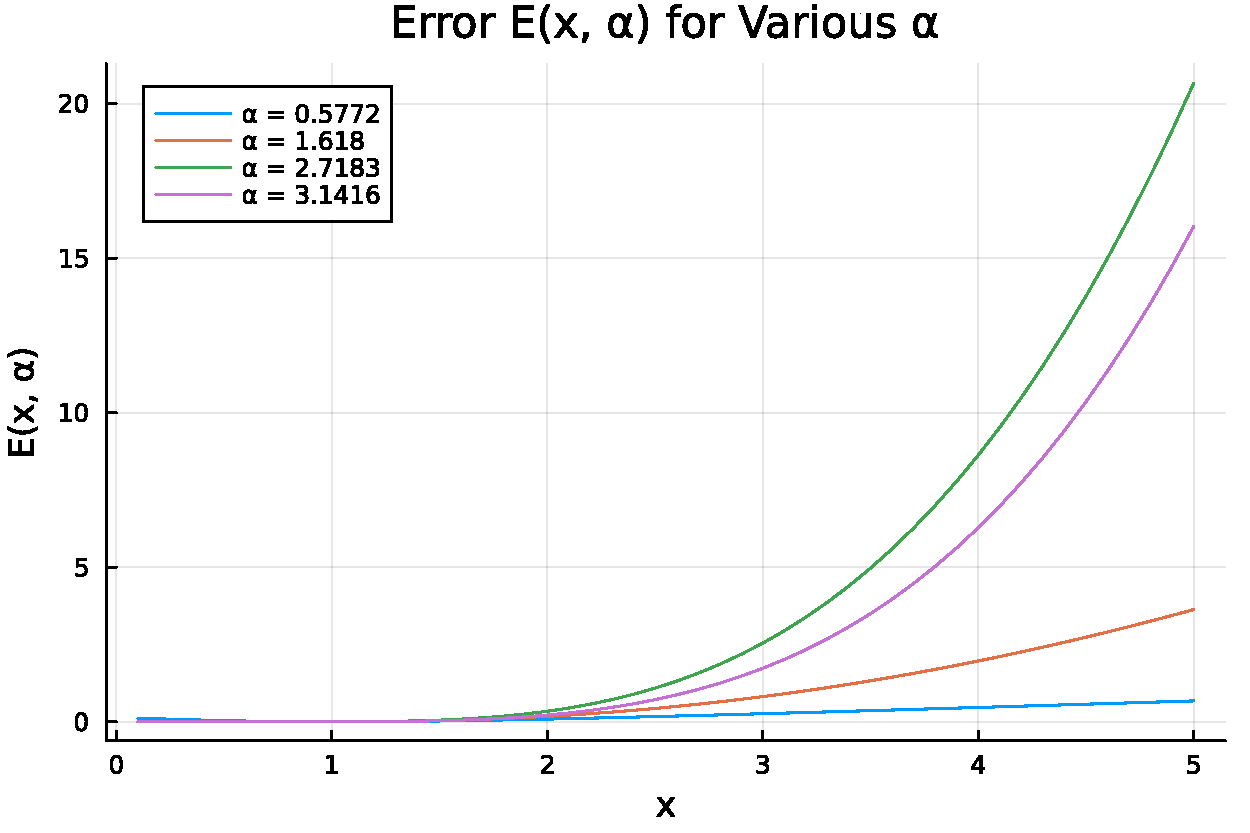
\includegraphics[width=0.7\textwidth]{figures/error_plot.pdf}
    \caption{Error of Caputo-Fabrizio MGF}
    \label{fig:error_MGF}
\end{figure}
It can be observed from figure \ref{fig:error_MGF} above that, in general for greater orders \(\alpha\), the error tends to increase. However, the greatest order of \(\alpha\) does not provide the greatest error. Instead it is the second greatest order of \(\alpha\) that does so. This may be explained by the fact that for values of \(\alpha\), being exactly in the middle of two integers, the value of \((1 - \beta)x + \beta\) will be the greatest. As a result, the fraction becomes small, so the error tends to increase.

This hypothesis is indeed confirmed in the following figure, which focuses on the growth rate of the error, for a fixed value of \(x\) and an increasing order \(\alpha\).

\begin{figure}[H]
    \centering
    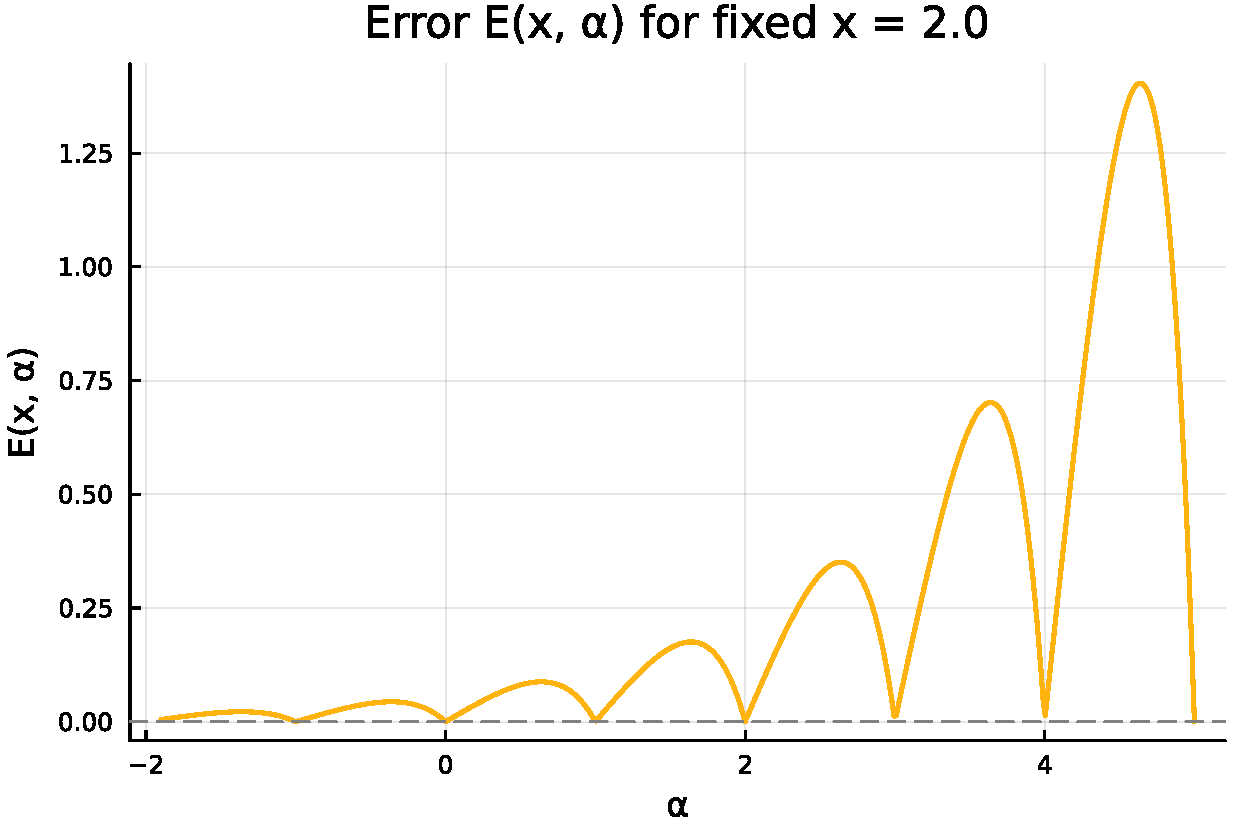
\includegraphics[width=0.7\textwidth]{figures/error_plot_fixed_x.pdf}
    \caption{Error of Caputo-Fabrizio MGF, for fixed x}
    \label{fig:error_MGF_fixed_x}
\end{figure}
Figure \ref{fig:error_MGF_fixed_x} indeed seems to indicate that for some \(\alpha \in (a, b)\), where \(a, b \in \mathbb{Z}\) are consecutive integers that \(E(x, \alpha)\) attains it maximum value for some \(\alpha\) 'slightly greater' than \(\frac{a + b}{2}\). Figure \ref{fig:error_MGF_fixed_x} also reveals that the approximation error is considerably smaller for negative fractional moments compared to the positive ones. This suggests that, when negative moments are well-defined, the Caputo-Fabrizio MGF might still offer reasonable accuracy, despite its known limitations.

Note that within each integer interval, the function \(E(x, \alpha)\) appears to be concave. Thus, as is supported by figure \ref{fig:error_MGF_fixed_x}, it is only possible to obtain local maxima. Ideally, one would aim to analytically determine the optimal order \(\hat{\alpha}\) such that minimizes \(E(x, \hat{\alpha})\). However, due to the concavity of \(E(x, \hat{\alpha})\), such analytical minimization is not feasible. Figure \ref{fig:error_MGF_fixed_x} seems to suggest that order of \(\alpha\) near integer orders yields smaller approximation errors, which makes sense intuitively. However, the latter is not rigorous evidence. Therefore, in the following section, we will analyse the numerical approximation errors of the Caputo-Fabrizio MGF by simulation. We will use numerical methods to try to obtain values \(\alpha\) which minimize the expression from theorem \ref{t: MGF_inaccurate}.

We have seen in the previous section how the error \(E(x, \alpha) = x^\alpha - \displaystyle \frac{x^{n+1} }{(1 - \beta)x + \beta}\) changes with increasing values of \(\alpha\). Now, we focus on the entire expression, as stated in theorem \ref{t: MGF_inaccurate}.
\subsection{Practical Issues}
Computing these expressions poses some difficulties. In the first place, we want to compute the moment of fractional order \(\alpha\) for a random variable \(X\). Julia does not have any packages to compute raw moments of such an order, thus these methods will have to be created first. In order to accomplish the desired result, we directly compute \(\int_{-\infty}^{\infty} x^\alpha  f_X(x) dx\). If the support of the random variable is infinite, this integral is often not numerically well defined. Thus, in such cases we use a bounded support \((-1000, 1000)\) which provides a sufficient accurate approximation. What is more, for many fractional orders \(\alpha\) in combination with negative values of \(x\), \(x^\alpha\) is of complex form. To avoid such expressions, given that the distribution is symmetric, we simply integrate the PDF over its non-negative support and factor the final value by 2. In this manner, it is still possible to obtain fractional moments of distributions such as the Normal distribution. If a distribution has a negative support and is not symmetric, it is possible to compute the complex or absolute moment of fractional order, which avoids any numerical issues. This approach, however, lacks interpretability, as the intuition behind absolute and complex moments is harder to grasp. 
\newline
It now remains to compute the fractional moment using the Caputo-Fabrizio MGF. Unfortunately, it is rather difficult to compute the fractional derivative of an MGF expression numerically. The reason is, that programming packages often take (fractional) derivatives on a certain point \(x\) rather than over the entire function. Thus, we simply use the result obtained in theorem \ref{t: MGF_inaccurate}. That is, instead of the moment of order \(\alpha\), the Caputo-Fabrizio MGF computes the moment of order \(n+1\) divided by some variables dependent on \(\alpha\). More explicitly, we compute \(\leftindex_{CF}{M}_X^{(\alpha)}(0) = \displaystyle \int_{-\infty}^{\infty}  \frac{x^{n+1} }{(1 - \beta)x + \beta} f_X(x)\). This integral faces the same problems as the aforementioned integral with \(x^\alpha\). What is more, for specific values of \(x\) and \(\beta\), the denominator tends to go towards zero, which is numerically unstable. Thus, in such cases, we add a rather small \(\epsilon\) in order to avoid this issue.

\subsection{Accuracy Analysis}\label{ss:accuracy_analysis}
For this accuracy analysis we consider different parameter values and orders of \(\alpha\). We set \(\alpha \in [0, 5]\) with steps of 0.01. This yields 500 errors per parameter-configuration, which provides us with a viable sample to analyse the characteristics of the errors. Whenever possible, we extend \(\alpha\) to the interval \((-1, 0)\). We consider three distributions, namely the Exponential, Normal and Poisson distribution. This selection allows us to cover both continuous and discrete distributions, distributions with negative and positive supports and symmetric distributions.
The observant reader might notice that all of the errors in the upcoming sections are non-negative and may incorrectly conclude that these are the absolute or squared errors. This is not the case. In each case we compute the expression obtained in theorem \ref{t: MGF_inaccurate}, for a different distribution. Since the expression \(E(x, \alpha) = x^\alpha - \displaystyle \frac{x^{n+1} }{(1 - \beta)x + \beta}\) is always non-negative, it follows that \( \displaystyle x^\alpha \geq \frac{x^{n+1} }{(1 - \beta)x + \beta}\) and thus \(\displaystyle \int_{-\infty}^{\infty} x^\alpha  f_X(x) dx \geq  \displaystyle \int_{-\infty}^{\infty}  \frac{x^{n+1} }{(1 - \beta)x + \beta} f_X(x) dx\) for any distribution, such that the expression from theorem \ref{t: MGF_inaccurate} is always non-negative.
\subsubsection{Exponential Distribution}
First we consider the Exponential distribution with PDF as defined in Appendix \ref{s:app_common_distributions}.
The support of the Exponential distribution is \([0, \infty)\), thus the integration process will avoid most numerical issues. Moreover, all relevant moments of the Exponential distribution are based on raw moments, which is precisely the kind of moments we are interested in.
\newline
We obtain the following figure:
\begin{figure}[H]
    \centering
    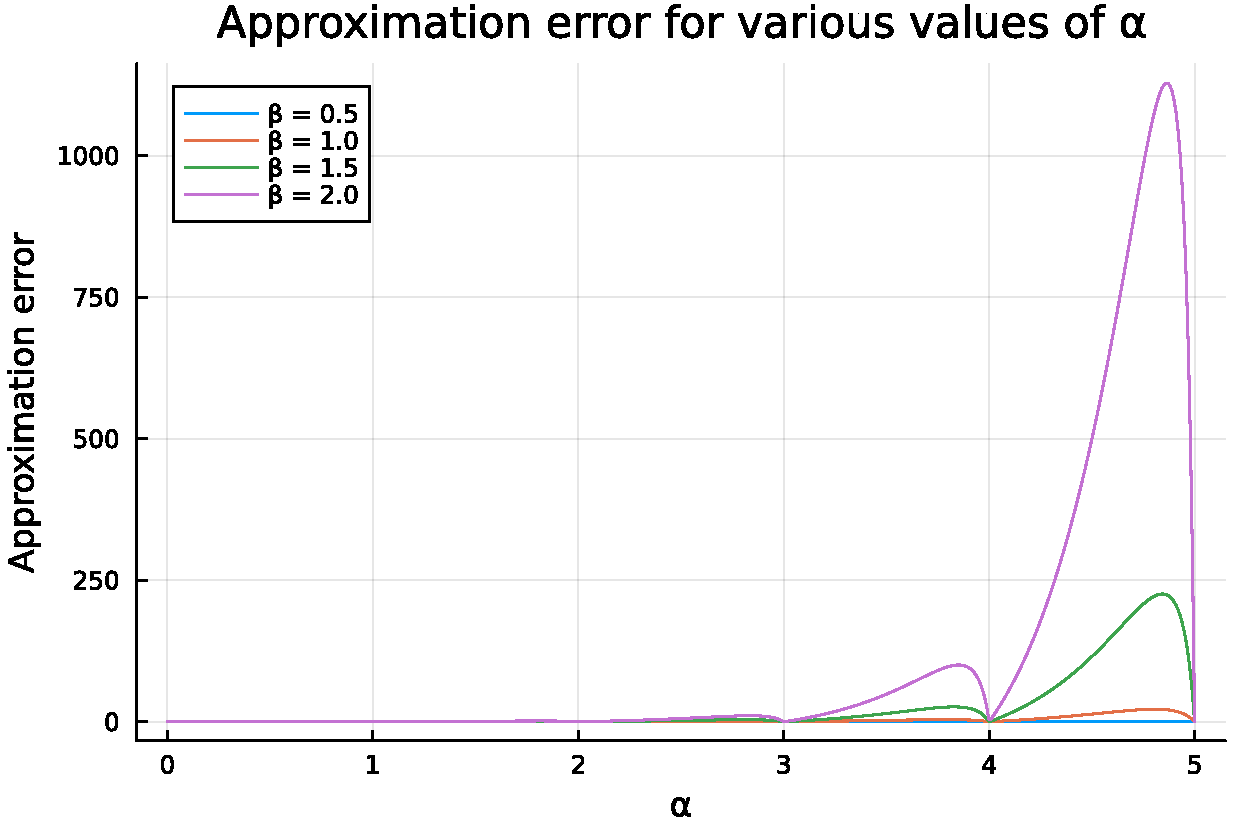
\includegraphics[width=0.7\textwidth]{figures/error_plot_exp.pdf}
    \caption{Approximation error for the Exponential Distribution}
    \label{fig:error_plot_exp}
\end{figure}
From figure \ref{fig:error_plot_exp}, it is clear that for a greater parameter value \(\beta\) the approximation error increases. Namely, for moments of higher order \((\alpha \geq 3)\), the approximation error increases rapidly. For smaller orders of \(\alpha\) the approximation errors remain relatively low. In practice, moments of order \(\alpha > 4\) are oftentimes not of interest. Thus, the greatest approximation errors will be avoided.

We obtain the following associated table with some core statistics:
\begin{table}[H]
    \centering
\begin{tabular}{ccccccc}
  \toprule
  \textbf{\(\beta\)} & \textbf{minimum} & \textbf{maximum} & \textbf{mean} & \textbf{standard deviation} & \textbf{skewness} & \textbf{\(c_v\)} \\\midrule
  0.5 & 0.0 & 0.329 & 0.074 & 0.083 & 1.762 & 1.12 \\
  1.0 & 0.0 & 22.119 & 2.907 & 5.612 & 2.314 & 1.93 \\
  1.5 & 0.0 & 225.731 & 25.477 & 54.91 & 2.513 & 2.155 \\
  2.0 & 0.0 & 1128.26 & 115.489 & 265.154 & 2.655 & 2.296 \\\bottomrule
\end{tabular}

\caption{Exponential Distribution - Approximation Error Statistics} 
\label{tab:exp_error}
\end{table}

The results in table \ref{tab:exp_error} align with the conclusions derived in figure \ref{fig:error_plot_exp}. The greater the values of \(\beta\) and order of \(\alpha\), the greater the (average) approximation error. For all values of \(\beta\), the minimum error is zero, which occurs when \(\alpha \in \mathbb{N}\). An interesting observation is that for \(\beta = 1.5\) the average approximation error exceeds the maximum approximation error for \(\beta = 1.0\). For all values of \(\beta\), the skewness is positive, implying that the distribution of the approximation errors is right-skewed. Thus, clearly the distribution of the errors is not symmetric and therefore certainly not a Normal distribution. In the last column, the Coefficient of Variation has been reported, which has been given by the formula \(\displaystyle \frac{\sigma}{\mu}\), where \(\mu\) and \(\sigma\) denote the sample and sample standard deviation respectively \cite{hendricks1936}. This metric of measurement allows us to objectively compare the variability of the errors of each of the parameter configurations. The lower \(c_v\), the lower the variability and thus the more consistent the dataset. This consistency is something we strive for, as it allows us to describe our data with greater confidence. From table \ref{tab:exp_error}, it is clear that the Coefficient of Variation increases as the parameter \(\beta\) increases. For \(\beta = 0.5\) all result are reasonable. The Caputo-Fabrizio MGF in combination with the Exponential(0.5) could still be viable in practice. For Exponential(1), this conclusion may depend on the maximum order of \(\alpha\).

\subsubsection{Normal Distribution}
We now consider \(X\) to be Normally distributed with mean \(\mu\) and standard deviation \(\sigma\), as defined in Appendix \ref{s:app_common_distributions}. This distribution is of particular interest as it has two parameters. Thus, we can analyse the differences of effect of both parameters on the approximation error. Therefore, while raw fractional moments of the Normal distribution are not commonly used in practice, we can still obtain valuable insights from this simulation.  The Normal distribution is symmetric with domain \(x \in \mathbb{R}\). So, we integrate the PDF over the interval \((0, 1000)\) to avoid numerical issues.
\newline

We obtain the following figure:
\begin{figure}[H]
    \centering
    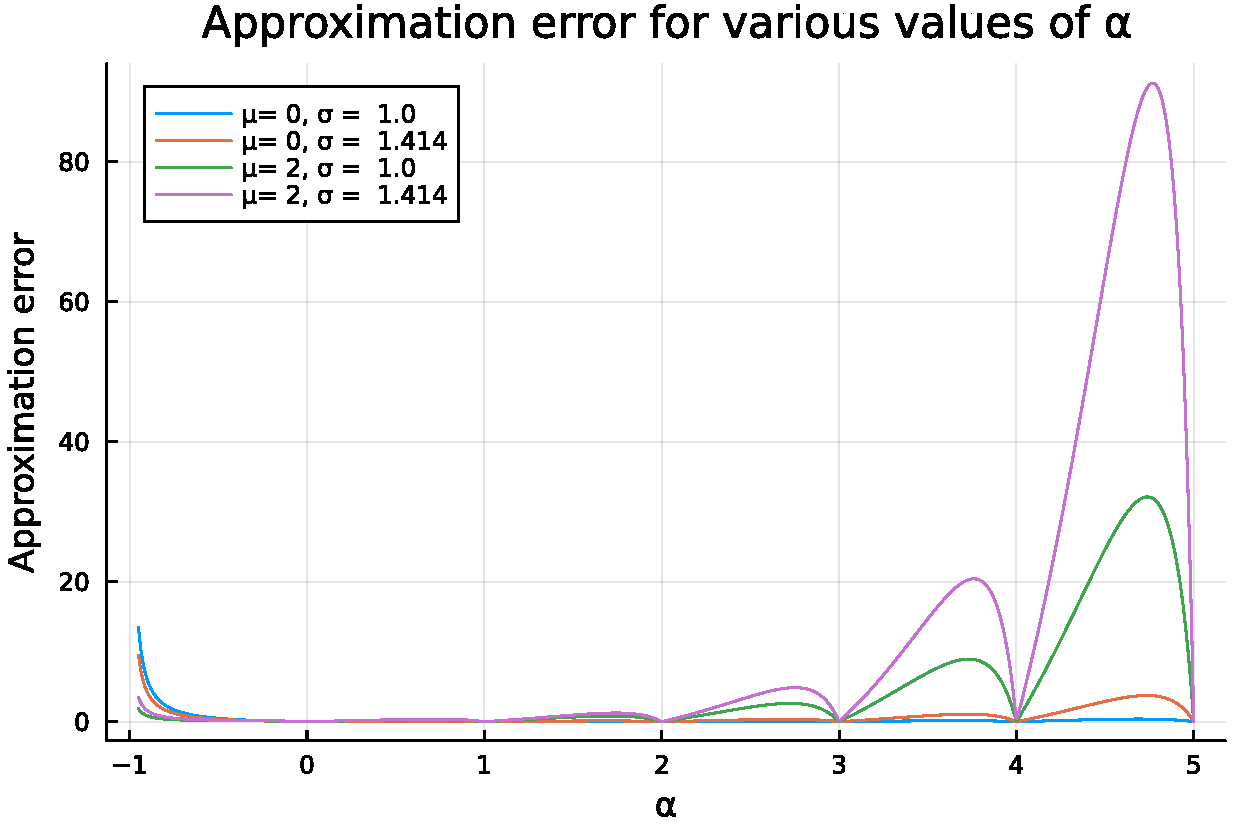
\includegraphics[width=0.8\textwidth]{figures/error_plot_normal.pdf}
    \caption{Approximation error for the Normal Distribution}
    \label{fig:normal_plot_error}
\end{figure}
As illustrated in figure \ref{fig:error_plot_exp}, the approximation error increases with \(\mu\) and \(\sigma\). This result is consitent with the result obtained for the Exponential distribution. However, the magnitude of the errors of the Normal distribution is considerably smaller. Furthermore, the figure also displays the errors for order \(\alpha \in (-0.95, 0)\). These errors tend to attain the same size as errors for order \(\alpha\) near 3. Interestingly, for negative orders of \(\alpha\), the effect of the parameter values seems to reverse. Larger values of \(\mu\) and \(\sigma\) are associated with smaller approximation errors.
\newline 

We obtain the following associated table with some core statistics:
\begin{table}[H]
    \centering
\begin{tabular}{cccccccc}
  \toprule
  \textbf{\(\mu\)} & \textbf{\(\sigma\)} & \textbf{minimum} & \textbf{maximum} & \textbf{mean} & \textbf{standard deviation} & \textbf{skewness} & \textbf{\(c_v\)} \\\midrule
  0.0 & 1.0 & 0.0 & 13.439 & 0.298 & 1.07 & 7.898 & 3.591 \\
  0.0 & 1.414 & 0.0 & 9.505 & 0.7 & 1.141 & 2.824 & 1.629 \\
  2.0 & 1.0 & 0.0 & 32.123 & 4.517 & 8.055 & 2.269 & 1.783 \\
  2.0 & 1.414 & 0.0 & 91.231 & 11.411 & 22.404 & 2.428 & 1.963 \\\bottomrule
\end{tabular}

\caption{Normal Distribution - Approximation Error Statistics} 
\label{tab:normal_error}
\end{table}
The statistics in table \ref{tab:normal_error} support the visuals conclusions drawn from figure \ref{fig:normal_plot_error}. The average of the approximation error for \(\mu = 0\) is acceptable. However, the size of its Coefficient of Variation compared to the other parameter configurations is remarkable. Indeed, configuration \((\mu, \sigma) = (0, 1)\) and configuration \((\mu, \sigma) = (0, \sqrt{2})\) have a rather similar standard deviation, however, the latter has approximately twice the average error. Except for this case, \(c_v\) again tends to increase as the parameter values increase, suggesting higher variability in approximation errors. Similar to the Exponential distribution, for all parameter-configurations, the distribution of the errors is right-skewed. Thus, the approximation errors of a Normal distribution are not Normally distributed themselves! This result is confirmed in figure \ref{fig:error_histogram}. Even in the histogram of the parameter-configuration with the greatest parameter values, more than 50 percent of the approximation errors cluster around zero, with only a small number of observations falling in the range \((40, 80)\). As before, the average errors and variability for large parameters may be too great to be reliable depending on the context of the application.

\begin{figure}[H]
    \centering
    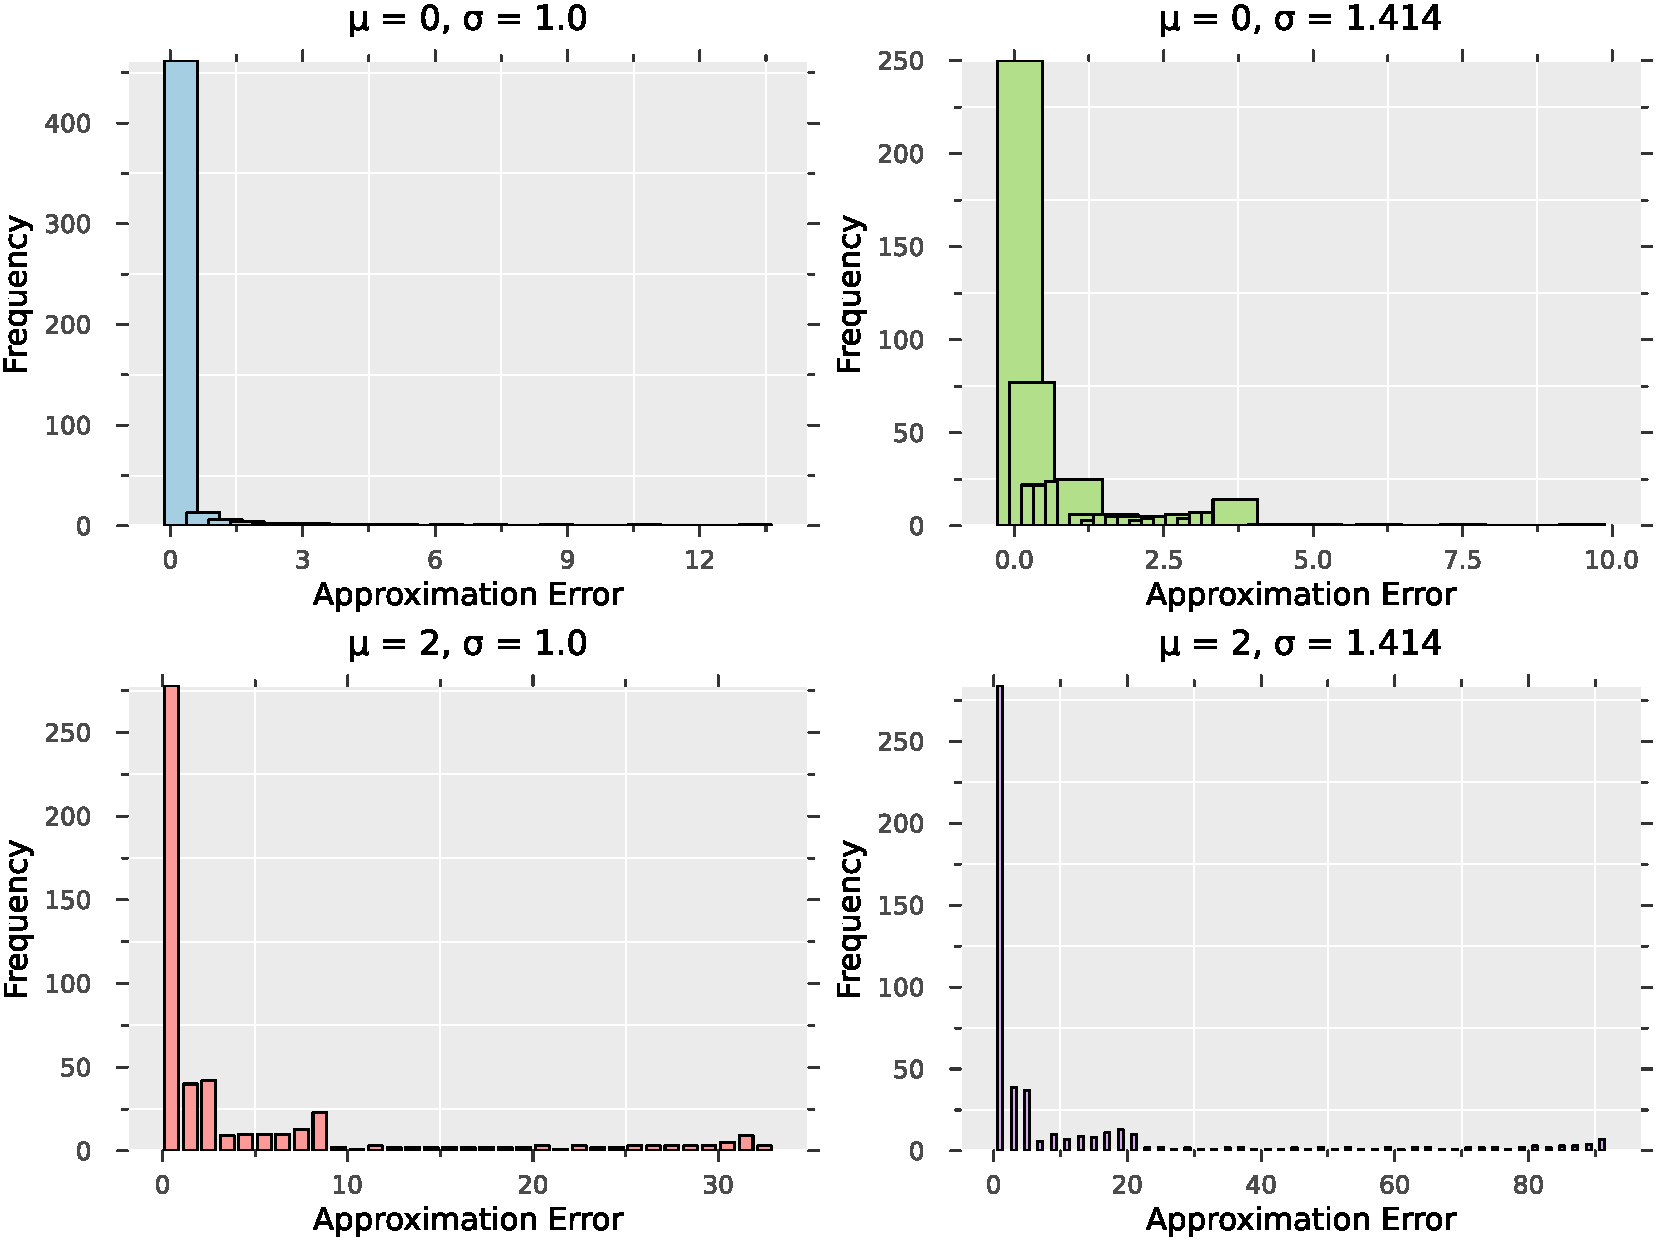
\includegraphics[width=0.83\textwidth]{figures/error_histogram.pdf}
    \caption{Error Histogram for the Normal Distribution}
    \label{fig:error_histogram}
\end{figure}

\subsubsection{Poisson Distribution}
Finally, we consider a discrete distribution to explore if these results differ from those of the continuous distributions. Specifically, we let \(X \sim Poisson(\lambda)\), with the probaility mass function defined as in Appendix \ref{s:app_common_distributions}. The Poisson distribution has positive support and its raw moments are given by: \[\mathbb{E}[X^k] = \sum_{i = 0}^{k} \lambda^i \stirlingii{k}{i}\] with \(k \in \mathbb{N}\) and where \(\{\}\) denotes the Stirling numbers of the second kind (rather similar to the binomial coefficient) \cite{haight1967}. This formula highlights that we cannot consider moment of negative order, as the expression relies on factorials and other combinatorial terms.

We obtain the following figure:
\begin{figure}[H]
    \centering
    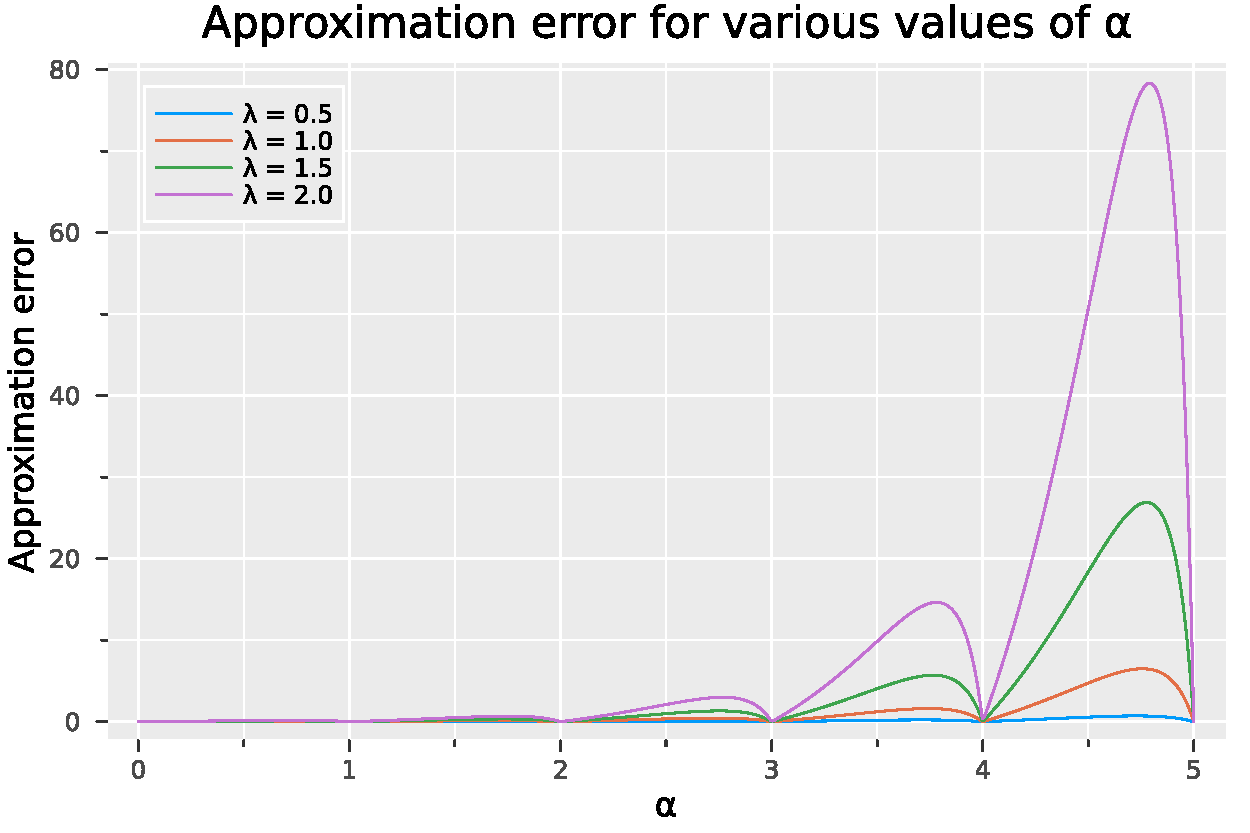
\includegraphics[width=0.7\textwidth]{figures/error_plot_poisson.pdf}
    \caption{Approximation error for the Poisson Distribution}
    \label{fig:poisson_plot_error}
\end{figure}
As shown in figure \ref{fig:poisson_plot_error}, the general trend of the Caputo-Fabrizio MGF errors in the case of the Poisson distribution, is consistent with that observed for continuous functions. Larger values of \(\lambda\) lead to greater approximation errors. The magnitude of the errors is comparable to that of the Normal distribution, and increases significantly for \(\alpha \geq 3\).


\begin{table}[H]
    \centering
\begin{tabular}{ccccccc}
  \toprule
  \textbf{\(\lambda\)} & \textbf{minimum} & \textbf{maximum} & \textbf{mean} & \textbf{standard deviation} & \textbf{skewness} & \textbf{\(c_v\)} \\\midrule
  0.5 & 0.0 & 0.715 & 0.128 & 0.191 & 1.915 & 1.494 \\
  1.0 & 0.0 & 6.5 & 1.021 & 1.713 & 2.075 & 1.679 \\
  1.5 & 0.0 & 26.904 & 3.895 & 7.001 & 2.176 & 1.797 \\
  2.0 & 0.0 & 78.34 & 10.687 & 20.143 & 2.251 & 1.885 \\\bottomrule
\end{tabular}

\caption{Poisson Distribution - Approximation Error Statistics} 
\label{tab:poisson_error}
\end{table}
The statistics in table \ref{tab:poisson_error} further support this conclusion.
As with previous distributions, the distribution of the errors is right-skewed and the Coefficient of Variation increases as the parameter, \(\lambda\), grows.
For \(\lambda = 0.5\) and \(\lambda = 1.0\), we can still obtain reliable computations. For \(\lambda = 1.5\), the results are still potentially viable, depending on the application and the importance of higher-order fractional moments. In order to minimize its associated standard deviation, one can consider a smaller maximum order of \(\alpha\). In contrast, the configuration \(\lambda = 2.0\) is likely to be too unreliable in practice, especially for order \(\alpha > 3\).

\begin{figure}[H]
    \centering
    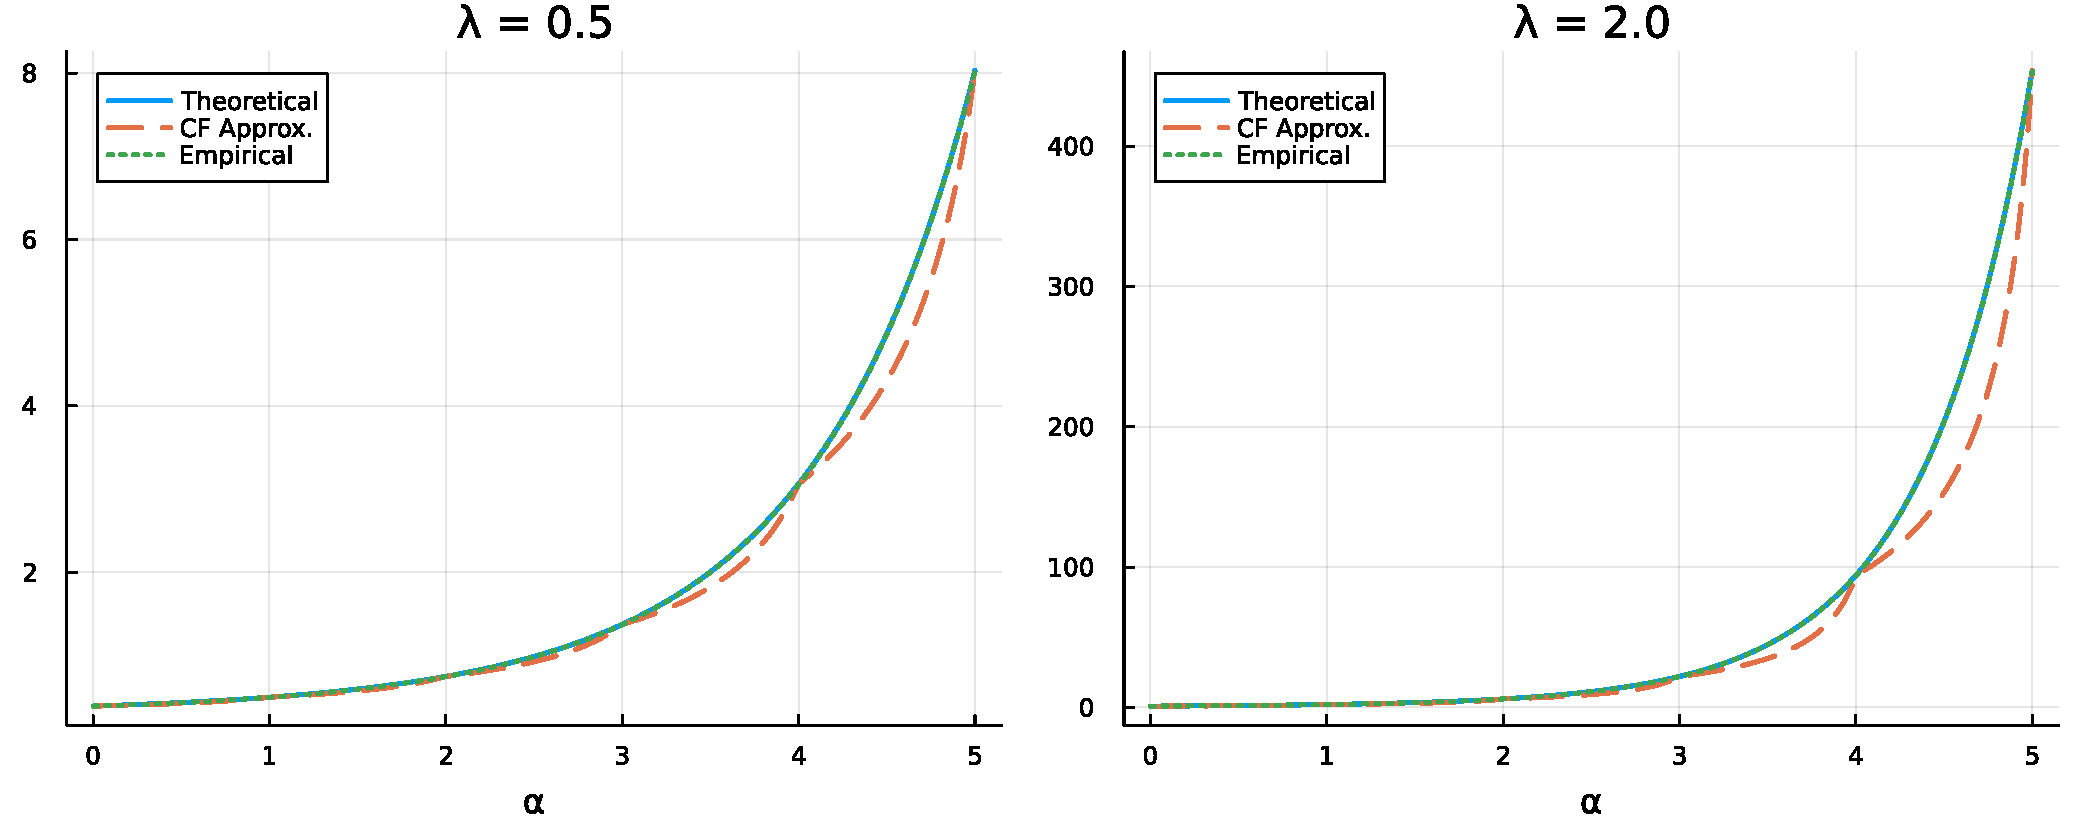
\includegraphics[width=1.0\textwidth]{figures/value_comparison.pdf}
    \caption{Comparison of different fractional moments for the Poisson Distribution}
    \label{fig:poisson_plot_values}
\end{figure}
The figure above depicts the values of fractional moments for various orders \(\alpha\) and \(\lambda \in \{0.5, 2.0\} \) as computed using the Caputo-Fabrizio MGF, the two accurate MGFs and the an empirical method. The latter takes a million random samples of the Poisson distribution and computes the mean of order \(\alpha\). The values of the accurate MGFs (blue line) and empirical values (dashed green-line) almost completely agree, confirming the accuracy and useability of the former. The values obtained by the Caputo-Fabrizio MGF are always smaller or equal to the values of the accurate MGF expressions. This observation is in line with the result that the errors are always non-negative. Note that, when the parameter \(\lambda\) becomes 4 times as great, the values of the fractional moments increase by more than 50 times their size. This again confirms that the approximation errors increase as the parameter values increase.

\subsection{General results}
Based on the three distributions analysed, we arrive at the following  general conclusions:
\begin{itemize}
    \item As the parameter value of the underlying distribution increases, both the average and maximum approximation error tend to increase.
    \item For all distributions considered, higher parameter values, lead to greater standard deviations in the approximation errors.
    \item Furthermore, the Coefficient of Variation also increases with larger parameter values, indicating that the standard deviation increases at a higher rate than the mean - a stronger result than the increase in the standard deviation alone.
    \item For all considered distributions and parameter values, the distribution of the approximation errors is right-skewed. Thus, we can conclude that the latter does not follow a Normal, or any other symmetric, distribution.
\end{itemize}
These findings raise important considerations regarding the reliability of the Caputo-Fabrizio MGF in practice. While high parameter values often result in a large Coefficient of Variation, suggesting that the quality of the approximation may behaves inconsistently, figure \ref{fig:error_histogram} offers a different perspective. Namely, in the case of the Normal distribution, at least 50 percent of the errors are clustered around zero. Most importantly, in this section, we are considering a sample of approximation errors of 500 fractional moments. When applying moments of fractional order in practice such as in \cite{hansen2024}, \cite{Mikosc2013} or \cite{gyzl2013}, one usually computes no more than five moments. Considering the latter, metrics such as the standard deviation and Coefficient of Variation may not always be relevant or decisive when evaluating the usability of the Caputo-Fabrizio MGF. Therefore, rejecting a parameter configuration solely based on its high variability may be too strict. In general, as long as the fractional order of the moment remains below 3 or is close to an integer, the Caputo-Fabrizio MGF tends to yield sufficiently accurate results. This supports its viability in practical cases, such as in \cite{hansen2024}, where only fractional moments of relatively low order are of interest.

\section{Practical Case}\label{s:practical_case}
To demonstrate the usage of the Moment Generating Function for computing moments of fractional order, we consider a dataset containing the weekly S\&P 500 index from the second week of January 2000 up until the last week of December 2024, provided by Wharton Research Data Services.
\subsection{First look at the data}
 The following figure depicts the trend of the S\&P 500 index over time:

\begin{figure}[H]
    \centering
    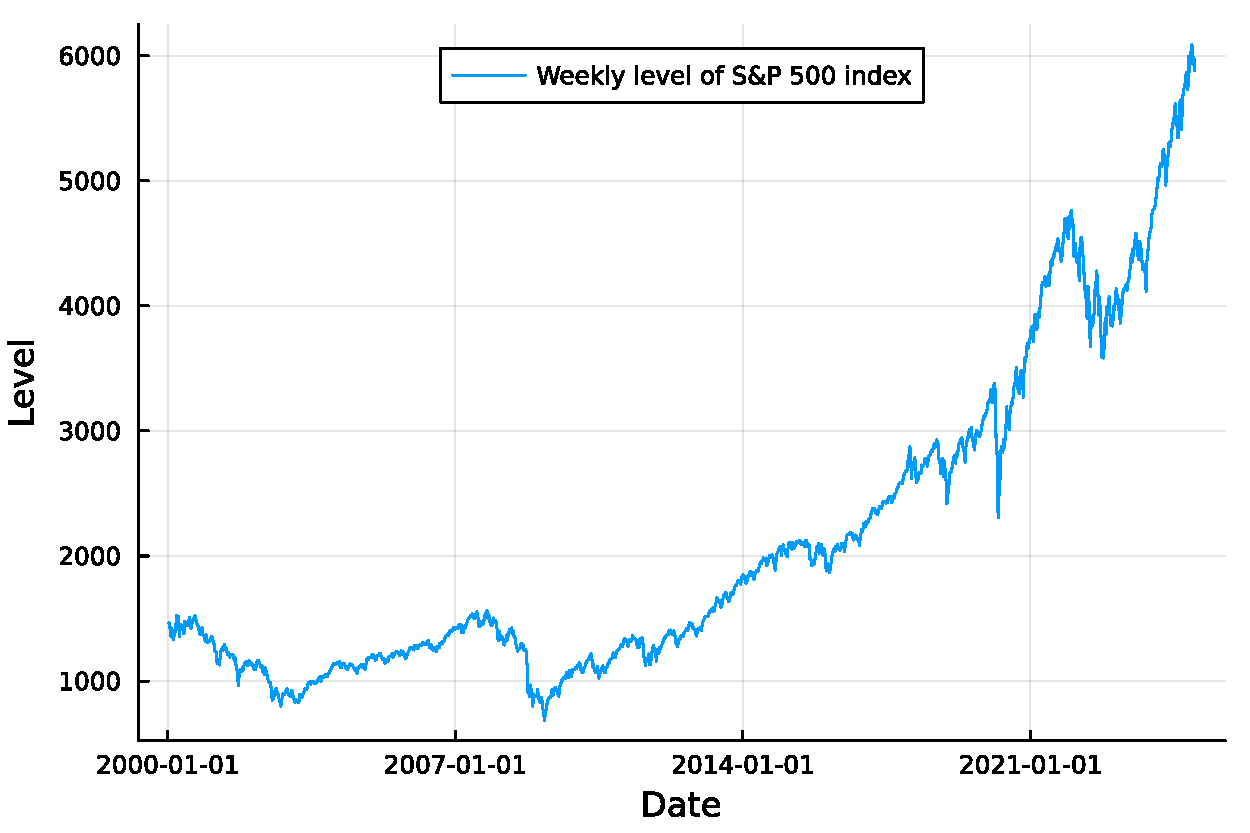
\includegraphics[width=0.7\textwidth]{figures/stock_level.pdf}
    \caption{S\&P 500 level over time}
    \label{fig:stock_level}
\end{figure}
It is clear from figure \ref{fig:stock_level} that the S\&P 500 index is non-stationary, as the mean of the process is not constant. We prefer to work with data that is stationary, thus we consider the log-returns (variations in stock-price) as shown in figure \ref{fig:stock_returns}. These values have been scaled by a factor of 100 to express them as percentages

\begin{figure}[H]
    \centering
    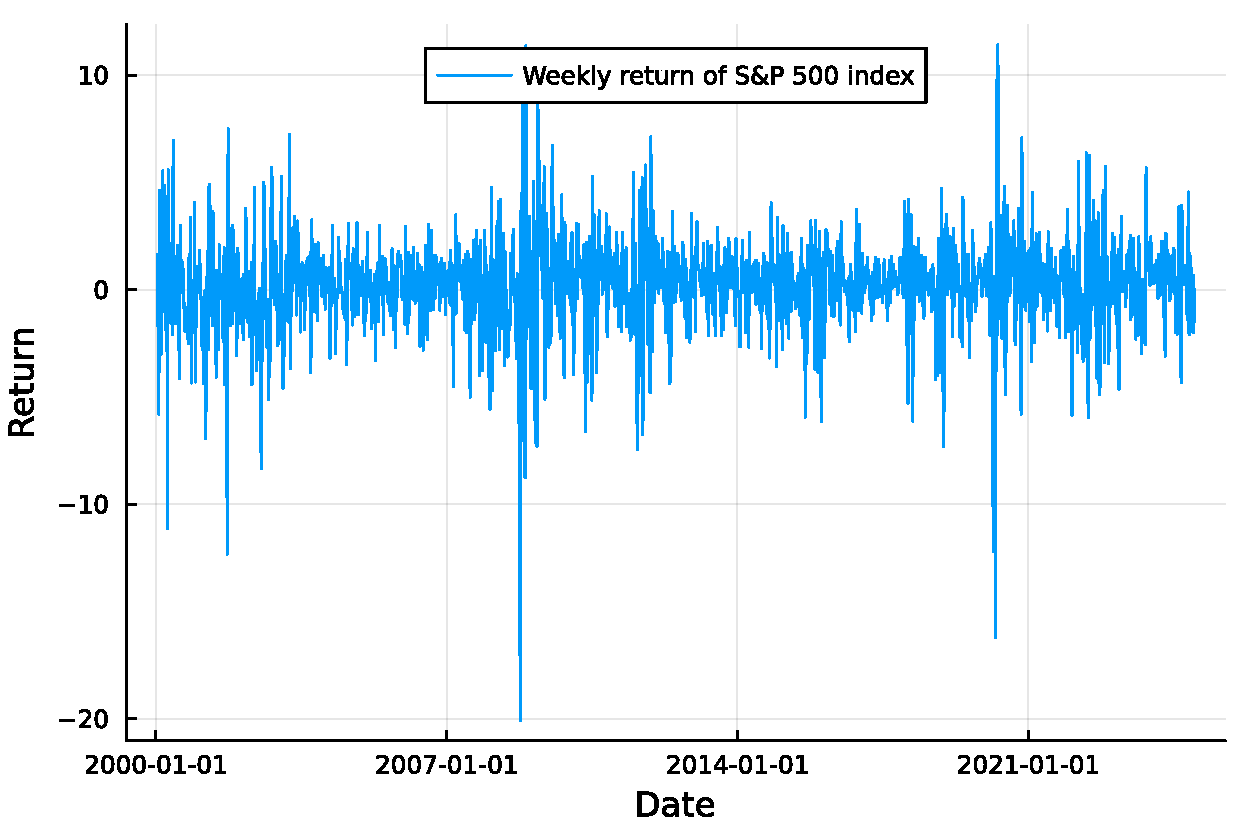
\includegraphics[width=0.7\textwidth]{figures/stock_returns.pdf}
    \caption{S\&P 500 log-returns over time}
    \label{fig:stock_returns}
\end{figure}
The log-returns series appears more suitable for volatility analysis compared to the data displayed in figure \ref{fig:stock_level}. The mean of the log-returns seems to be stationary (lying around zero), the variance of the log-returns also seems to remain constant over time. Additionally, there are no signs of seasonality. Notable spikes in the log-returns around 2008 and 2021 likely correspond the global financial crisis and COVID pandemic respectively. In times of (financial) uncertainty, it is more likely that returns may take more extreme values, making them less predictable.
\newline

The following core statistics of the log-returns, as displayed in figure \ref{fig:stock_returns} have been computed:

\begin{table}[H]
    \centering
\begin{tabular}{ccccc}
  \toprule
  \textbf{Mean} & \textbf{Variance} & \textbf{Skewness} & \textbf{Kurtosis} & \textbf{P-value}\\\midrule
  0.108 & 6.17 & -0.878 & 7.225 & 1e-99 \\\bottomrule
\end{tabular}

\caption{Summary Statistics log-returns of S\&P 500} 
\label{tab:summary_statistics}
\end{table}
Indeed, as anticipated, the (unconditional) mean seems to be around zero. Moreover, the rather great value of the kurtosis in table \ref{tab:summary_statistics} indicates that the log-returns of the S\&P 500 are not normally distributed, as this value is far greater than 3 which is expected in the context of financial markets, due to frequent occurrence of extreme values. The normal distribution, known for its thin tails, underestimates the probability of such extremes. The p-value included in table \ref{tab:summary_statistics} is the associated p-value of the augmented Dickey-Fuller unit root test, with null hypothesis: the log-returns of the s\&P 500 stock index is a unit root process.  The p-value is so small that we reject the hypothesis at any conventional significance level. Thus, we can formally conclude that the weekly log-returns of the S\&P 500 index are stationary.

\subsection{Modelling volatility of the log-returns}
It is well known that the stock prices, as well as the mean of log-returns, cannot be predicted. Therefore, we focus on the volatility of the log-returns instead. A widely used approach is the autoregressive conditional heteroskedasticity model of order \(q\), denoted ARCH(q), introduced by \cite{engle1982}. With observation equation: 
\begin{equation}
    r_t = \sigma_t \cdot \epsilon_t
\end{equation}

and updating equation:

\begin{equation}
    \sigma^2_t = \omega + \sum_{i = 1}^{q} \alpha_i \cdot r^2_{t-i}
\end{equation}

Another commonly used model is the Generalized Conditional Heteroskedasticity model of order \((p, q)\), denoted GARCH(p, q), as proposed by \cite{bollerslev1986} with observation equation

\begin{equation}
    r_t = \sigma_t \cdot \epsilon_t 
\end{equation}

and updating equation:

\begin{equation}
    \sigma^2_t = \omega + \sum_{i = 1}^{p} \beta_i \cdot \sigma^2_{t-i} + \sum_{i = 1}^{q} \alpha_i \cdot r^2_{t-i}
\end{equation}
To determine which model is more appropriate for monitoring volatility, we first examine the autocorrelation function (ACF) of the data. The ACF of log-returns is typically close to zero, and is therefore considered to be negligible in practice. Instead, we analyse the autocorrelation function of the squared log-returns.
The following figure depicts the autocorrelation function of the squared log-returns (note that the first index at \(t = 0\) has been removed as \(corr(r_i, r_j)\) is always equal to 1 for \(i = j\)).

\begin{figure}[H]
    \centering
    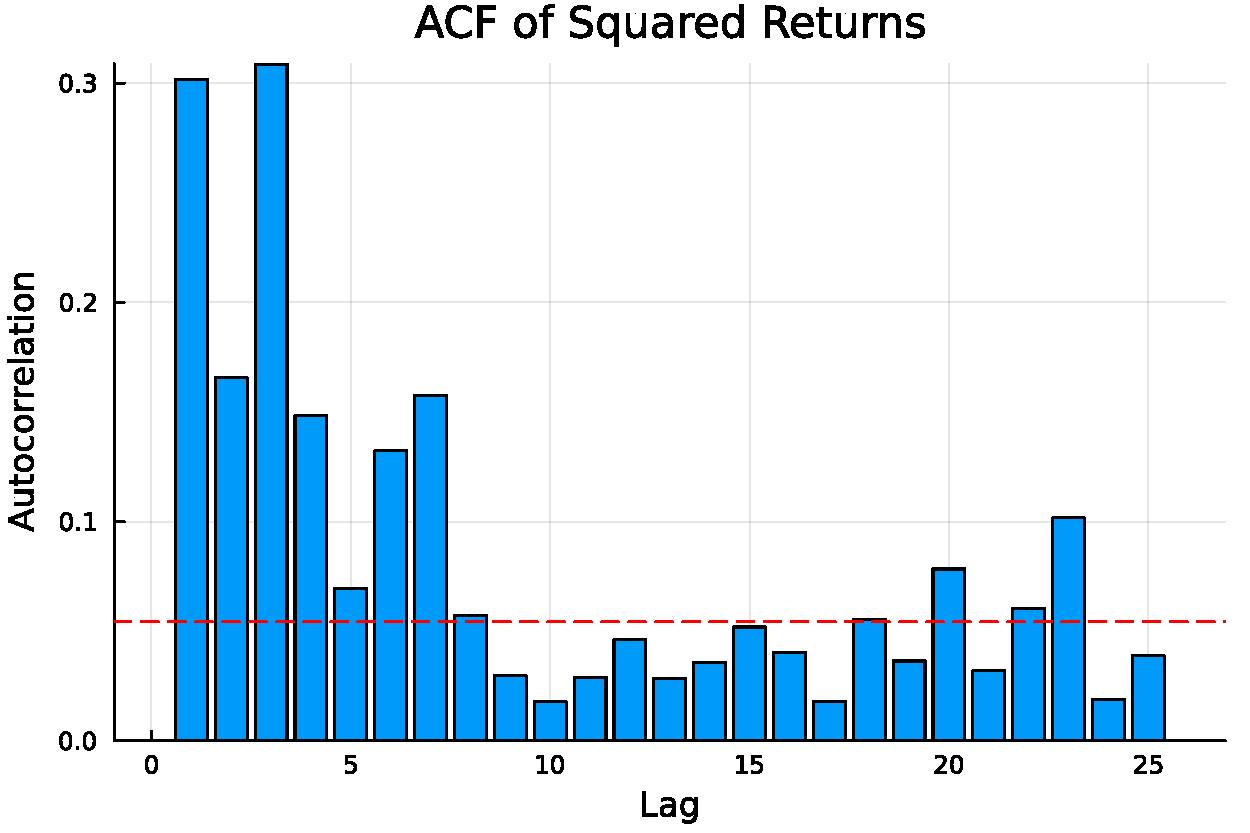
\includegraphics[width=0.7\textwidth]{figures/acf_squared_returns.pdf}
    \caption{ACF of Squared log-returns}
    \label{fig:acf_squared_returns}
\end{figure}

From figure \ref{fig:acf_squared_returns} we observe that a substantial number of lags exhibit autocorrelations exceeding the 95\% confidence interval (given by the red dashed line). This suggests that autocorrelation function does not decay exponentially and that an ARCH(1) model would be inadequate for describing the volatility in this dataset. Consequently, we GARCH\((p, q)\) model. We opt for the latter, as choosing the former often leads to too many parameters to estimate.

To determine the number of parameters \(p\) and \(q\) such that the GARCH\((p,q)\) model describes the volatility of the data the best, we compute the Akaike information criterion (AIC) and the Bayesian information criterion (BIC). The model having both the lowest AIC and BIC value is to be preferred. We consider GARCH\((p, q)\) models for \(p, q \in \{1, 2, 3\}\).

\begin{table}[H]
    \centering
\begin{tabular}{ccc}
  \toprule
  \textbf{Model} & \textbf{AIC} & \textbf{BIC} \\\midrule
  GARCH(1,1) & 5699 & 5714 \\
  GARCH(1,2) & 5700 & 5721 \\
  GARCH(1,3) & 5697 & 5723 \\
  GARCH(2,1) & 5700 & 5721 \\
  GARCH(2,2) & 5702 & 5728 \\
  GARCH(2,3) & 5699 & 5730 \\
  GARCH(3,1) & 5702 & 5727 \\
  GARCH(3,2) & 5703 & 5734 \\
  GARCH(3,3) & 5699 & 5735 \\\bottomrule
\end{tabular}

\caption{AIC and BIC for GARCH models} 
\label{tab:aic_bic}
\end{table}

From table \ref{tab:aic_bic} we observe that the GARCH(\(1, 3\)) model achieves the lowest AIC value, while the GARCH(\(1, 1\)) has the lowest BIC value. Both models also obtain relatively low values for the other criterion, indicating that they are good candidates for modeling volatility. For simplicity, we proceed with the GARCH\((1, 1)\) model as that means we will only need to estimate three parameters instead of five, leading to more straightforward interpretability.

The parameters have been estimated using Maximum Likelihood Estimation. Link functions were applied to ensure non-negativity of the parameters and that the log-returns form a weakly stationary white noise process.

\begin{table}[H]
    \centering
\begin{tabular}{ccc}
  \toprule
  \textbf{Parameter} & \textbf{Estimate} & \textbf{Standard error} \\\midrule
  \(\omega\) & 0.37 & 0.084 \\
  \(\alpha\) & 0.224 & 0.030 \\
  \(\beta\) & 0.726 & 0.031 \\\bottomrule
\end{tabular}

\caption{Parameter Estimates of GARCH(1,1)} 
\label{tab:parameter_estimates}
\end{table}

Indeed, \(\hat{\alpha} + \hat{\beta} < 1\) confirming that the log-returns represent a weakly stationary white noise sequence. Moreover, the standard errors of the estimates are relatively small, indicating high precision.


\subsection{Using fractional moments to analyse the log-returns}
Now that we have described the data using core statistics, fitted appropriate models and estimated their parameters, we finally consider the usage of moments of fractional order to enhance the analysis.
\subsubsection{Computing conditional absolute moments of fractional order}\label{sssec:conditional_fractional_moments}
Following \cite{hansen2024}, we compute the conditional expectation of the absolute variance over a given period \(H\), specifically
\[\mathbb{E}[|X_{T + H}|^\gamma \mid \mathcal{F_T}],\]
 where \(X_{T+H} = Var(R_{T, H}) = \mathbb{E}[R_{T, H}^2] = \mathbb{E}[\sum_{t = T + 1}^{T + H} r_t^2] = \sum_{t = T + 1}^{T + H}\mathbb{E}[ r_t^2] \). Here \(r_t\) denotes the log-return at time \(t\) and \(\mathcal{F_T}\) represents the natural filtration, which is the sigma-algebra generated by the process up to time \(T\) \cite{lowther2009}. In other words, \(\mathcal{F_T}\) contains all information about log-returns observed up to time \(T\). Note that \(Var(R_{T, H})\) is indeed equal to \(\mathbb{E}[R_{T, H}^2]\) as \(\mathbb{E}[R_{T, H}]^2 = \mathbb{E}[\sum_{t = T + 1}^{T + H} r_t]^2 = \left(\sum_{t = T + 1}^{T + H} \mathbb{E}[r_t]\right)^2\). We assume that \(r_t \sim \mathcal{N}(0, \sigma^2_t)\) and since the autocorrelation function of log-returns is zero, we have that each \(r_t\) is independent of the observations at different time indices. So it follows that: \(\left(\sum_{t = T + 1}^{T + H} \mathbb{E}[r_t]\right)^2 = \left(\sum_{t = T + 1}^{T + H} 0\right)^2 = 0\). To avoid confusion, we denote the order of the fractional moment by \(\gamma\) rather  than \(\alpha\) which is already used as a parameter in the GARCH(1,1) model. We compute moments of order \(\gamma \in \{-0.5, 0.5, 1.5, 2\}\) as suggested by \cite{hansen2024}.
According to \cite{hansen2024} the orders of \(\gamma\) correspond to the following moments:

\begin{itemize}
\item \(\gamma = -0.5\): Inverse of the volatility of the returns. May be used for Sharpe ratio forecasting
\item \(\gamma = 0.5\): Conditional volatility or standard deviation of  returns
\item  \(\gamma = 1.5\): Conditional skewness (of the absolute value)
\item  \(\gamma = 2\): Conditional kurtosis
\end{itemize}

These fractional methods are computed using three different methods. 
\begin{itemize}
\item \textbf{Empirical Simulation: } We consider the empirical value of the moments, obtained by performing 100.000 Monte Carlo simulations of the distribution of the variance (see algorithm \ref{alg:simulate_conditional_variance}) followed by averaging the results to obtain the empirical estimates.
\item \textbf{Integral method: } We compute the standard integral, namely \(\int_{-\infty}^{\infty} (x)^\gamma f_X(x) \, dx\), where \(f_X(x)\) is the PDF of \(X_{T,H}\). This PDF is acquired by performing Kernel Density Estimation on the values of \(X_{T,H}\).
\item \textbf{Caputo-Fabrizio MGF: } We also compute the expectations of fractional order using the inaccurate method of the Caputo-Fabrizio MGF. This integral also makes use of the same PDF obtained by Kernel Density Estimation.
\end{itemize} 

We compute these moments for different time horizons, namely \(H \in \{4, 8, 16\}\). That is, we compute the expectation of the absolute variance of order \(\gamma\) for one month, two months and four months in the future, respectively. This allows us to evaluate whether the time horizon affects the performance of the Caputo-Fabrizio method. The full procedure is detailed in algorithm \ref{alg:analyse_fractional_moments}.

We obtain the following table:


\begin{table}[H]
    \centering
\begin{tabular}{ccccc}
  \toprule
  \textbf{H} & \textbf{order} & \textbf{empirical} & \textbf{standard} & \textbf{CF} \\\midrule
  4 & -0.5 & 0.25 & 0.255 & 0.138 \\
  4 & 0.5 & 4.948 & 4.938 & 1.855 \\
  4 & 1.5 & 201.653 & 201.763 & 56.748 \\
  4 & 2.0 & 1568.7 & 1569.69 & 1569.69 \\
  8 & -0.5 & 0.164 & 0.164 & 0.06 \\
  8 & 0.5 & 7.098 & 7.095 & 1.94 \\
  8 & 1.5 & 552.323 & 552.142 & 114.85 \\
  8 & 2.0 & 5909.13 & 5905.96 & 5905.96 \\
  16 & -0.5 & 0.113 & 0.113 & 0.028 \\
  16 & 0.5 & 10.073 & 10.066 & 1.971 \\
  16 & 1.5 & 1550.63 & 1547.5 & 230.747 \\
  16 & 2.0 & 23559.0 & 23482.6 & 23482.6 \\\bottomrule
\end{tabular}

\caption{Conditional expectations for various orders} 
\label{tab:conditional_expectations}
\end{table}
The results from table \ref{tab:conditional_expectations} can be interpreted as follows:

\begin{itemize}
\item \(\gamma = -0.5\): The inverse of the volatility decreases with \(H\), implying that the volatility increases as the forecast horizon extends. All values are positive, due to use of absolute moments.
\item \(\gamma = 0.5\): The standard deviation of the returns indeed increase when the value of \(H\) increases. This is expected as greater time horizons lead to more uncertainty.

\item  \(\gamma = 1.5\): The conditional skewness greatly increases when the value of \(H\) increases. However, since we examine the absolute value, all skewness values are positive, making the interpretability limited.

\item  \(\gamma = 2\): The conditional kurtosis vastly increases as the value of \(H\) increases. For all values of \(H\), the kurtosis is considerably greater than 3, implying that the conditional absolute cumulative returns are not normally distributed. As with skewness, the interpretability is limited due to the use of absolute values.
\end{itemize}

For all values of \(H\) and non-integer values of \(\gamma\) the empirical results and  theoretical  integral results are closely aligned. Similarly, for all values of \(H\) and \(\gamma = 2\), the results of the integral method and Caputo-Fabrizio MGF are the same, as the latter is accurate for integer derivatives of the MGF. As indicated in section \ref{s:simulation}, the Caputo-Fabrizio MGF greatly under-estimates the values of fractional moments. These errors increase with \(H\), implying that the method increasingly underestimates volatility - and hence risk - for longer horizons. We therefore conclude that the Caputo-Fabrizio MGF is unreliable for computing expectations of fractional order in forecasting applications. This conclusion is consistent with the results of section \ref{ss:accuracy_analysis}, where the size of the errors grew as the distribution parameters increased. Figure \ref{fig:conditional_moments_error} emphasizes the increment of the errors of the Caputo-Fabrizio MGF.



\begin{figure}[H]
    \centering
    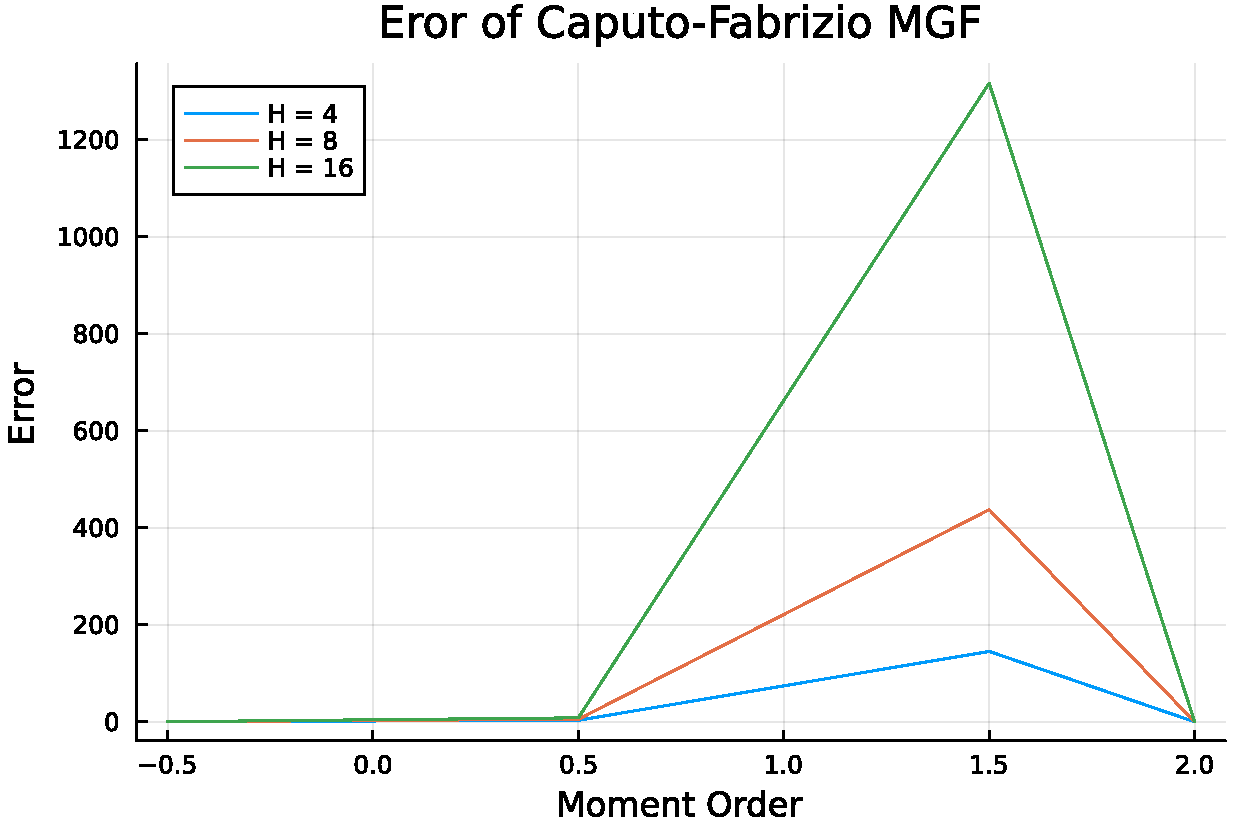
\includegraphics[width=0.7\textwidth]{figures/conditional_moments_error.pdf}
    \caption{Error of Caputo-Fabrizio MGF for various values of \(H\) and \(\gamma\)}
    \label{fig:conditional_moments_error}
\end{figure}\

Note that figure \ref{fig:conditional_moments_error} only includes discrete values of \(\gamma \in \{-0.5, 0.5, 1.5, 2\}\). Therefore, the plotted functions may give a misleading impression of continuity. For instance, the error at \(\gamma = 1\) should be exactly zero, yet the graph figure suggests otherwise due to the interpolation between points.

\subsubsection{More about the computation and interpretability of fractional moments}
An observant reader might wonder why we compute the expectation of \(| X_{T + H}|\) instead of simply computing the expectation of \( X_{T + H}\). We have that \(X_{T+H} = Var(R_{T,H}) \geq 0\) so why are these absolute values necessary? The answer is twofold. When we are computing moments of negative order, i.e. \(\gamma = -0.5\) we are computing a function that behaves similar to \(\displaystyle \frac{1}{\sqrt{X_{T+H}}}\). It is quite clear that this computation will suffer from numerical issues for variances in a neighbourhood of zero. The second reason lies in the manner of how we compute the standard and CF-MGF moments. As aforementioned there exists no simple analytical expression of the MGF in this context ( \cite{hansen2024} managed to find one, but considered a different model to monitor volatility, which seemed to be outside of the scope of this thesis). Thus we need to work with a PDF of \(X_{T+H}\). To obtain this density, we use Kernel Density Estimation (KDE), which may occasionally produce negative values, especially around the tails of the distribution, where there are less data points. Computing negative values of fractional order is not well-defined, thus in this case, we have to include absolute values as well. As seen in table \ref{tab:conditional_expectations}, this may result in values that are less intuitive or interpretable. We could also have considered to give a complex form to \(X_{T+H}\) allowing for negative values. However, these results are most likely even less intuitive. Another option would have been to square all orders to ensure that the integral is well defined for all values of the PDF. This would lead to all orders being integer orders again, which defeats the purpose of considering moments of fractional orders in the first place.

\subsubsection{Analyzing risks using VaR and fractional orders of LPM}
Next, we consider two different measures of risk, namely the Value-at-Risk (VaR) measure and the Lower Partial Moment (LPM). Where the former is defined as 
\begin{equation}
    \alpha\text{-VaR} = z_\alpha \cdot \sigma_{t + H} 
\end{equation}
 where \(z_\alpha\) is the quantile of level \(\alpha\) of the standard normal distribution \cite{holton2013}.
While VaR focuses on a single quantile threshold, LPMs may provide a more complete picture of downside risk by capturing the magnitude as well as the frequency of returns falling below a specific target. The LPM is defined as follows:

\begin{equation}
    LPM_n(\tau) = \int_{-\infty}^{\tau} ( \tau - x)^n dF_X(x)
\end{equation}
 where \(\tau = \alpha\text{-VaR}\) and \(F_X(x)\) is the distribution of a random variable \(X\) \cite{wojt2009}. In our case \(X\) is the absolute cumulative return.  The intuition of the VaR is as follows: given some portfolio with a weekly \(\alpha-\text{VaR}\) of some percentage \(p\), there is a
probability of \(\alpha\)\% that the value of the portfolio will fall by more than \(p\)\% of its value in one week. The interpretation of the Lower Partial Moment, which is usually defined for \(n \in \mathbb{N}\) is as follows. The Lower Partial Moment of order \( n = 1\), is called the expected shortfall, which captures the expected downside deviation below the target value, \(\tau\). If the Lower Partial Moment is of order \( n = 0\), it represent the probability of performing under the target value, \(\tau\) \cite{sortino2001}. We extend the order of the Lower Partial Moment by letting \(n \in \mathbb{R}\), focusing on \( n \leq 1\), as proposed by \cite{fishburn1977}. According to the latter, the LPM of order \( 0 < n < 1\) emphasizes the frequency of downside incomes. The following figure depicts the Value-at-Risk with \(\alpha = 5\)\%, along with the Lower Partial Moment of order \(n \in \{0, 1, 0.5\}\), where \(LPM_{0.5}(\tau)\) has been computed using both the accurate and inaccurate expressions of the fractional MGFs. The risks are based on the forecasts of the cumulative returns up until H = 26, so half a year in advance.

\begin{figure}[H]
    \centering
    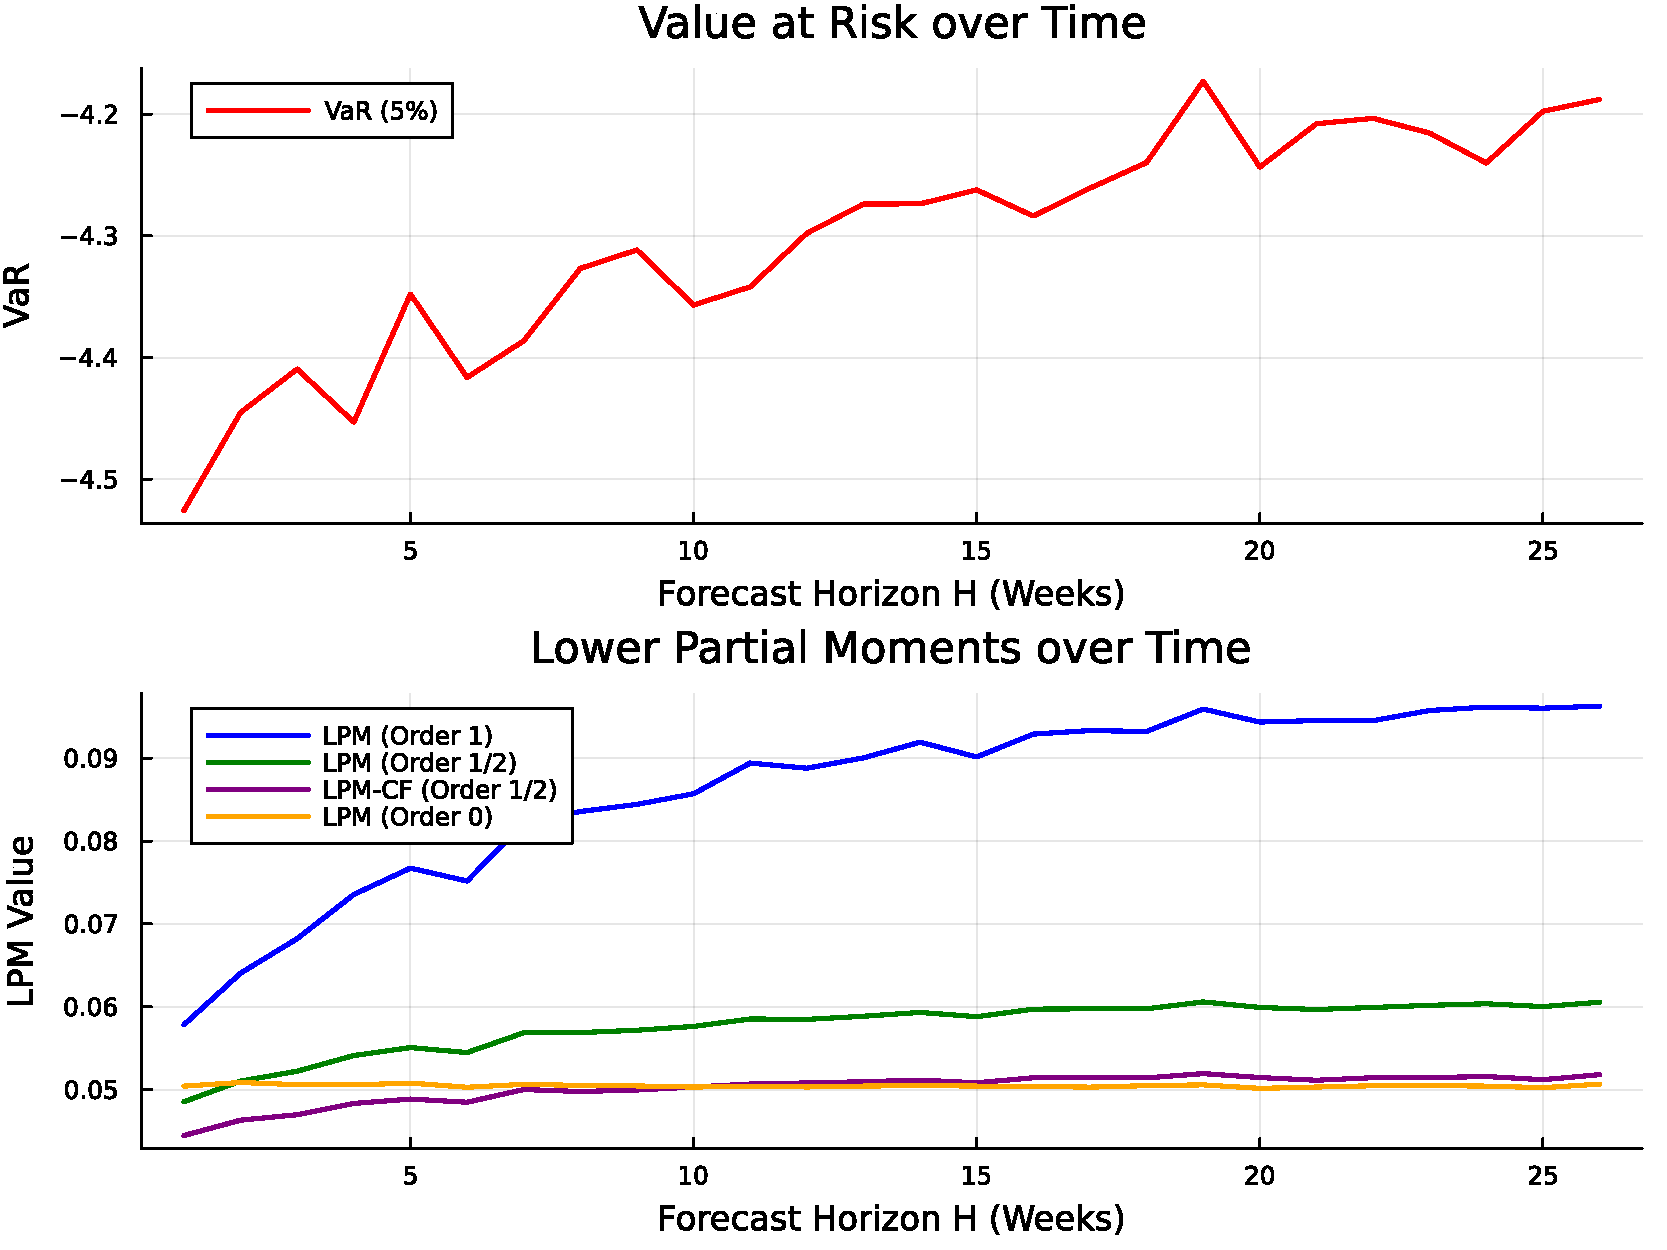
\includegraphics[width=1.0\textwidth]{figures/var_vs_lpm_alternative.pdf}
    \caption{Comparison of VaR and LPM for various orders of LPM}
    \label{fig:var_vs_lpm}
\end{figure}
\begin{itemize}
    \item From figure \ref{fig:var_vs_lpm} we observe that as \(H\) increases, the VaR quantile decreases in absolute magnitude, indicating that extreme losses become less severe relative to shorter horizons. This might seem counterintuitive at first, as stock returns may seem less predictable over larger periods of time, however this observation actually aligns theoretical expectations. That is \(\lim_{h \to \infty} \sigma^2_T(h) = \omega /(1 - \alpha - \beta)\). So as \(H\) increases, \(\sigma^2_T(h)\) will get closer to its unconditional variance and the function will become less steep.
\item As \(H\) increases, \(LPM_1(\tau)\) tends to increase slightly. This suggests that, while the expected downside loss below the threshold \(\tau\) may slightly increase over time, it does so at a decreasing rate. The flattening of the \(LPM_1(\tau)\) function reflects the convergence of the aforementioned unconditional variance which is in line with the theory of GARCH models.
\item As \(H\) increases, \(LPM_0(\tau)\) seems to follow the same trends as the other orders of \(LPM_n(\tau)\). The latter suggests that the downside risk grows marginally as time increases but eventually becomes constant. This is in line with the fact that return distributions converge to their long-run unconditional distribution as time increases.
\item \(LPM_{0.5}(\tau)\) seems to show a gradual increase, as \(H\) increases, after which it eventually flattens. This implies that the frequency and magnitude of downside deviations slowly grow over time and eventually reaching a maximum. The latter reflects the diminishing risk over long periods.
\item As concluded before, fractional moments computed by the Caputo-Fabrizio MGF, inaccurately underestimated. All values of \(LPM_{0.5}(\tau)\) computed via the Caputo-Fabrizio MGF are consistently lower than those computed using direct integration, once more conforming its systematic underestimation of downside risk. The Caputo-Fabrizio MGF approach does not fully capture the tail behaviour of the return distribution, especially for small values \(H\) where it even obtains smaller values compared to \(LPM_0(\tau)\).
\end{itemize}

\subsubsection{Modelling volatility using an observation-driven regression model}
In this final section, we try forecasting volatility using a different model. Namely, we consider an observation-driven regression model, a special case of the Generalized Autoregressive Score framework \cite{creal2013}.
This model has observation equation:
\begin{equation}
    y_t = \beta_t \cdot x_t + \epsilon_t
\end{equation}  
where \(\epsilon_t \sim \mathcal{N}(0, \sigma^2)\) and updating equation:

\begin{equation}
    \beta_t = \omega + \phi \cdot \beta_{t-1} + \alpha(y_{t-1} - \beta_{t-1}\cdot x_{t-1})x_{t-1}
\end{equation}
 This model has the advantage of allowing \(\beta_t\) to evolve over time, in contrast to models like GARCH(1,1) which impose a constant parameter structure. Such time-varying parameters are especially useful when working with financial return series that contain extreme values or structural changes. A fixed parameter may be overly influenced by outliers, whereas a dynamic \(\beta_t\) allows the model to adapt flexibly to such deviations without negatively affecting prediction accuracy. In our application, we let \(y_t\) represent the variance from one-month future returns. We will consider two different versions of the model.
\begin{itemize}
    \item Standard model: we let \(x_t = |r_t|\) represent the absolute return at time \(t\), as in \cite{taylor2007}.
    \item Extended model: we let \(x_t\) represent the conditional expectation of the absolute variance over two weeks of order 0.5. That is \(x_t = \mathbb{E}[|X_{T + 2}|^{0.5} \mid \mathcal{F}_t]\), with \(X_{T + 2}\) defined as before. This choice is motivated by section \ref{sssec:conditional_fractional_moments} where this value was interpreted as the standard deviation of the absolute returns over a period of two weeks.  
\end{itemize}
The goal of this specific case study is to compare the regression performance between a model with and without a moment of fractional order serving as regressor. In order to make sure we focus on this objective and do not get lost in an array of different definitions of fractional moments, we will only consider the fractional moments computed using the expression of the accurate MGFs. It is safe to say that comparing this fractional MGF with the standard model is a lot more useful than comparing a faulty MGF with the standard model.

The dataset has been split as follows: 80\% of the data has been used for the training-set and the remaining 20\% functions as the test-set. Around 50\% of the training-set has been reserved for estimating the parameters of the GARCH(1,1) model. We already estimated the parameters of a GARCH(1,1) model, but the estimates of those parameters were based on the entire dataset. In this case, we need parameter estimates for each different time \(t\) to obtain the most accurate computations of \(\mathbb{E}[|X_{T + 2}|^{0.5} \mid \mathcal{F}_t]\). We still make use of the parameters we estimated in \ref{tab:parameter_estimates} as we let \(\sigma^2_0 = \hat{\omega} / ( 1 - \hat{\alpha} - \hat{\beta})\) be the initial value of \(\sigma^2_t\). We compute \(\mathbb{E}[|X_{T + 2}|^{0.5} \mid \mathcal{F}_t]\) for all \(t\)-values in our selected window. The computation is rather similar to those of section \ref{sssec:conditional_fractional_moments}, with only a slight modification in the code (see algorithm \ref{alg:compute_z}).
After performing Maximum Likelihood Estimation, we obtain the following estimates:
\begin{table}[H]
    \centering
\begin{tabular}{ccccc}
  \toprule
  \textbf{Model} & \textbf{\(\hat{\omega}\)} & \textbf{\(\hat{\phi}\)} & \textbf{\(\hat{\alpha}\)} & \textbf{\(\hat{\sigma^2}\)} \\\midrule
  Standard model & 0.066 & 0.78 & 0.007 & 0.839 \\
  Extended model & 0.08 & 0.812 & 0.219 & 0.683 \\\bottomrule
\end{tabular}

\caption{Parameter Estimates of the two different regression models} 
\label{tab:observation_model}
\end{table}
The two models yield similar estimates for \(\omega\) and \(\phi\). 
The most notable differences appear in the parameter estimates of \(\hat{\alpha}\) and \(\hat{\sigma^2}\). The higher value of  \(\hat{\alpha}\) implies that the updates to \(\beta_t\) of the extended model are more responsive to the product of the past error term and regressor compared to the standard model, namely \(\epsilon_{t -1} \cdot x_{t-1}\). Meanwhile, the smaller value in the extended model \(\hat{\sigma^2}\) of \(\epsilon_{t-1} \sim \mathcal{N}(0, 0.683)\) compared to \(\epsilon_{t-1} \sim \mathcal{N}(0, 0.839)\) indicates reduced variance in the residuals, suggesting a better fit of the model. 

The following plot displays the path of \(\beta_t\) for the standard and extended model, that is, it shows the evolution of the value of \(\beta_t\) over the training period (2010-2022).

\begin{figure}[H]
    \centering
    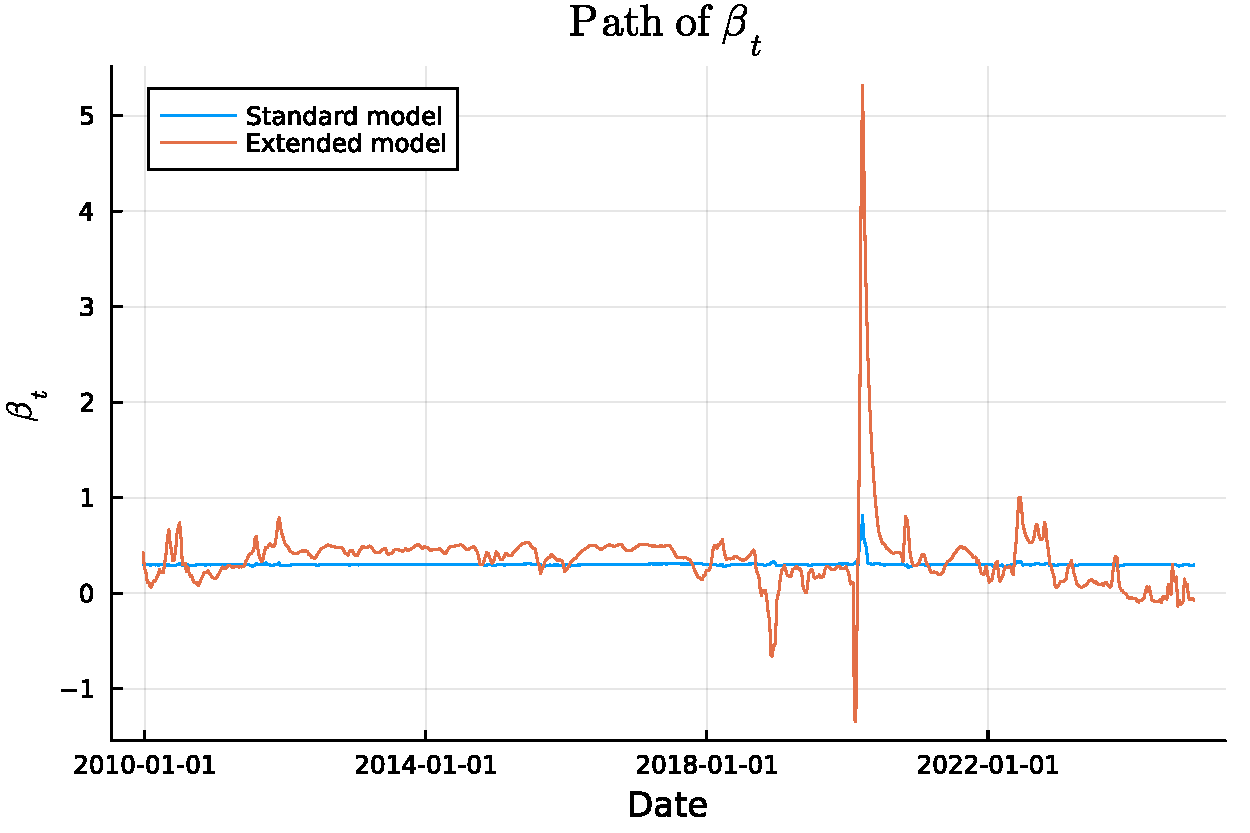
\includegraphics[width=0.7\textwidth]{figures/beta_path_alternative.pdf}
    \caption{Path of \(\beta\) for different models}
    \label{fig:beta_path}
\end{figure}
In the standard model \(\beta_t\) remains relatively stable, clustering around a value of 0.5, except for a spike around 2020 (COVID pandemic). In contrast, the extended model produces a more volatile \(\beta_t\) fluctuating between values around -1 and 5. This is possibly due to how \(\beta_t\) is updated in the extended model. Namely \(\beta_{T + 2}\) is dependent on \(\mathbb{E}[|X_{T + 1}|^{0.5} \mid \mathcal{F}_t]\). We have seen in section \ref{sssec:conditional_fractional_moments} how large these fractional moments can get. Therefore, as the value of \(\mathbb{E}[|X_{T + 1}|^{0.5} \mid \mathcal{F}_t]\) explodes, so will the value \(\beta_t\). The spike during the COVID pandemic perfectly illustrates this behaviour, where greater uncertainty drove up the value of the fractional moment and thus the value of \(\beta_t\).

The table below includes some performance measures of the standard model and extended model respectively.
\begin{table}[H]
    \centering
\begin{tabular}{ccccc}
  \toprule
  \textbf{Model} & \textbf{MSE} & \textbf{MAE} & \textbf{RMSE} & \textbf{\(R^2\)} \\\midrule
  Standard model & 0.275 & 0.387 & 0.524 & 0.023 \\
  Extended model & 0.207 & 0.349 & 0.454 & 0.267 \\\bottomrule
\end{tabular}

\caption{Performance measures of the two different regression models} 
\label{tab:performance_measures}
\end{table}
The values of the mean squared error, mean absolute error and root mean squared error of the extended model are all smaller compared to those of the standard model, indicating that the extended model is preferred. It also achieves a higher value for \(R^2\). Note that \(R^2\) is not always a reliable performance measure for time series data. This follows from the fact that in a time series context, there exists autocorrelation between the residuals, thus violating the assumption that residuals should be independent of each other. Using \(R^2\) in context of time series often results in low values of \(R^2\) indicating poor predictive performance, while this may not necessarily be the case. Yet, in table \ref{tab:performance_measures} we observe that the associated \(R^2\) value of the extended model is roughly ten times the value of the associated \(R^2\) value of the basic model. This suggests that the regressor \(x_t\) in the extended model has a much greater correlation with the variation in \(y_t\) compared to the regressor \(x_t\) in the standard model. That is, the regressor \(x_t\) in the extended model explains a greater portion of the variance in \(y_t\). Thus, in this context, the performance measure \(R^2\) is still found to be useful.
The following figure depicts the actual variance along with the variance predicted by the two different models:

\begin{figure}[H]
    \centering
    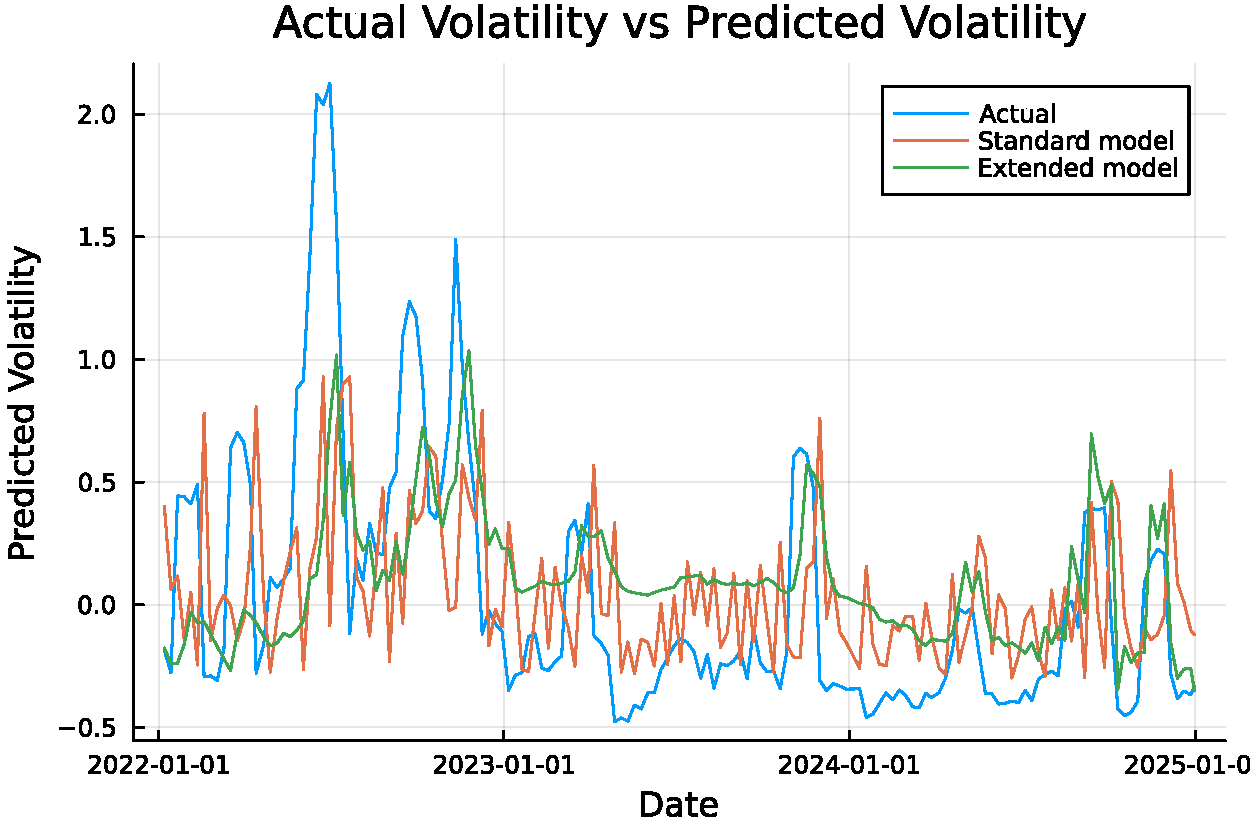
\includegraphics[width=0.7\textwidth]{figures/predicting_volatility.pdf}
    \caption{Actual volatility vs Predicted volatility}
    \label{fig:predicting_volatility}
\end{figure}
From figure \ref{fig:predicting_volatility} we observe that the actual variance attains more extreme values compared to the predictions. While the \(\beta_t\) value of the extended model was more flexible, as shown in figure \ref{fig:beta_path}, it is the predicted volatility of the standard model that fluctuates relatively more. The predicted volatility path of the extended model is much smoother, similar to the actual variances. This might explain the significant difference in performance measures between the two models. 

In conclusion, incorporating an expression involving fractional moments as a regressor leads to an improved performance in predictions of volatility. The extended model not only obtains lower prediction errors, but also better captures the structure of the data. This comes with an increase in volatility of the coefficient path, which may be either an advantage or disadvantage depending on the specific application. 

\section{Conclusion}\label{s:con}
This thesis has explored a relatively new method for computing moments of fractional order. This novel approach included combining the moment generating function with various different fractional derivatives. It was shown that the moment generating function in combination with either the Riemann-Liouville fractional derivative or the Grünwald-Letnikov fractional derivative leads to accurate computations of fractional moments. In contrast, the moment generating function in combination with the Caputo-Fabrizio fractional derivative leads to a consistent under-estimation of moments of fractional order.
It was shown that in general the mean and maximum error, the standard deviation, skewness and the coefficient of variation of the error increase as the parameter values of the underlying distribution grow. Nevertheless, the Caputo-Fabrizio moment generating function remains accurate for integer orders and in general, most of the errors are clustered around zero. 

The practical relevance of moments of fractional order was demonstrated through the application of volatility forecasting in financial markets. These moments were used to derive informative statistics for future stock returns and volatility. The values obtained using the Riemann-Liouville and Grünwald-Letnikov moment generating functions aligned closely with the empirical values, thus confirming their effectiveness in real world applications.

Additionally, the concept of lower partial moments was extended to fractional orders, which represent the frequency and magnitude of downside deviations. In both applications, the Caputo-Fabrizio moment generating function was shown to under-estimate the moments of fractional order. In particular when the forecasting horizon increased. This suggests that the Caputo-Fabrizio moment generating function is not well suited for financial risk analysis, as it tends to understate volatility and associated risk. 

Moreover, moments of fractional order were implemented as regressors in an observation-driven regression model. This approach allowed for a more flexible \(\beta_t\) compared to the \(\beta_t\) of the standard model, which led to reduced errors and improved forecasting accuracy compared to a standard model. In the absence of closed-form expressions of the moment generating function in this setting, it was required to make use of traditional numerical integration. To ensure numerical stability, absolute values had to be used, which leads to the computation of absolute moments of fractional order. While this is an effective solution, it limits the interpretability of the results, compared to unrestricted fractional moments. This limitation could be avoided if closed form expressions of the moment generating function are available.
\newline

Future research could include exploring moment generating functions in combinations with different fractional derivatives as those proposed by \citet{hadamard1892}, \citet{riesz1949} and \citet{marchaud1927}. It would be valuable to assess which combinations obtain accurate values of moments of fractional order and whether a general theorem regarding the accuracy of the moment generating function in combination with fractional derivatives can be established. Another topic of interest would be to consider computing fractional moments of multivariate distributions as briefly mentioned in \citet{hansen2024}. This would allow for computing fractional cross-moments to explore dependencies between different random variables. On a practical level, developing Julia packages capable of performing symbolic differentiation similar to SymPy in Python \citep{meurer2017} would reduce reliance on manual derivation. Currently, the lack of such tools in Julia requires all derivative expressions to be computed by hand before use, making computation an inefficient and painful process.







\section*{Acknowledgements}
I would like to thank my supervisor Gabriele Mingoli for the great guidance and clear and fast communication. I would like to thank \textbf{Person A}, \textbf{Person B} for peer reviewing my paper and \textbf{Person C}, \textbf{Person D} for the feedback on language, grammar and general structure.
\appendix

\section{Appendix: Relevant Functions and Identities}\label{s:appendices}

\begin{definition}\label{def:laplace}
    Let \(\displaystyle F(s) = \mathcal{L}(f) = \int_{0}^{\infty}e^{-st} f(t) dt\) be the Laplace transform of \(f\). Then \(f = \mathcal{L}^{-1}(f)\) is said to be the inverse Laplace transform of \(F\). The Laplace transform can be used to convert differential equations to much simpler algebraic equations \citep{thiagarajan2022}.
\end{definition}

\begin{definition}\label{def:mellin}
    The Mellin transform of some function \(f(t)\) is defined as \(\mathcal{M}\{f(t)\}(s) = \displaystyle \int_{0}^{\infty} t^{s-1} f(t) dt\). The Mellin transform is often used in computer science for the analysis of algorithms \citep{flajolet1996}.
\end{definition}

\begin{definition}\label{def:fourier}
    The Fourier transform of some function \(f(x)\) is defined as \(\displaystyle \hat{f}(\xi) = \int_{-\infty}^{\infty} f(x) e^{-2 \pi i \xi x}dx\), \(\xi \in \mathbb{R}\). The Fourier transform can be used to simplify differential equations and finds applications in signal and image processing \citep{fourier1822}. 
    
\end{definition}

\begin{definition}
    Let \(D\) be the differential operator, such that \(D f(x) = \frac{d}{dx} f(x)\). Then, as in \citet{samko1993}, the fractional derivative of order \(\alpha\) is defined as \[D^{\alpha} f(x) = \frac{d^{\alpha}}{dx^{\alpha}} f(x)\]
    
\end{definition}
In this definition, \(\alpha\) can be any real number. When taking regular derivatives, \(\alpha \in \mathbb{N}\). In most of our cases, we are interested in the instance where  \(\alpha \in \mathbb{R}_+\). It is also possible to study derivatives of negative order, which can be used to obtain moments of negative order of a random variable, provided that such an order exists. A derivative of negative order is simply an integral of positive order. This is defined as follows:
\begin{definition}
    Let \(I\) be the integral operator, such that \(I f(x) = \int f(x) dx\). Then by \citet{cauchy1823} the fractional integral of order \(\alpha\) is defined as \[(I^{\alpha} f) (x) = \frac{1}{(\alpha-1)!}\int (x-t)^{\alpha-1} f(t) dt\]
\end{definition} 

Combining the previous two definitions, we obtain the following, more general, definition, as in \citet{oldham1974}.
\begin{definition}\label{d: differintegral}
    The differintegral operator is defined as
    \begin{equation}
        R^\alpha f(x) = \begin{cases}
            I^{|\alpha|} f(x) & \text{if } \alpha < 0 \\
            D^\alpha f(x) & \text{if } \alpha > 0 \\
            f(x) & \text{if } \alpha = 0
        \end{cases}, \text{ with } \alpha \in \mathbb{R}.
        \end{equation}
        
\end{definition}

We define the (Euler-)Gamma function as follows:
\begin{definition}\label{d: eg}
    Let \(z \in \mathbb{C}\), for \(\Re(z) > 0\), we have the following: \(\displaystyle \Gamma(z) = \int_{0}^{\infty} t^{z-1} e^{-t} dt\)
\end{definition}

The Gamma function can be seen as an extension of the factorial function, for non-integers. This function is defined for complex numbers and all there subsets (so also real numbers), as long as the condition above holds. For positive integers values \(z\), we have the following identity: \(\Gamma(z) = (z - 1)!\)
Other important identities, not necessarily for \(z\) an integer, are: 
\begin{itemize}
    \item \(\Gamma(z + 1) = z \Gamma(z)\)
    \item \(\Gamma(2) = \Gamma(1) = 1\)
    \item \(\Gamma(\frac{1}{2}) = \sqrt{\pi}\)
\end{itemize}


\begin{definition}\label{def:binomial}
    For \(0 \leq k \leq n\), the Binomial Coefficient is defined as follows: \[\binom{n}{k} = \frac{n!}{k! (n - k)!} = \frac{\Gamma(n + 1)}{\Gamma(k + 1) \cdot \Gamma( n - k  + 1)}\] where \(n, k \in \mathbb{N}\) and \(\Gamma(.)\) as defined in \ref{d: eg}.
\end{definition}


\begin{definition}\label{def:vandermonde}
    Vandermonde's identity: for non-negative integers, \(k, l, m, n\), we have that \[\sum_{k = 0}^{l} \binom{m}{k} \cdot \binom{n}{l - k} = \binom{m + n}{l}\]
\end{definition}
A modification on the latter identity has been called the Chu-Vandermonde identity. This is the same identity, but it his been proven that the identities still hold for complex values \(m, n\) as long as \(l\) is a positive integer \citep{askey75}.

\begin{definition}\label{d: binomial}
    The binomial series is a generalization of the binomial formula, namely:
    \[(1 + x)^\alpha = \sum_{k = 0}^{\infty}\binom{\alpha}{k} \cdot x^k\]
\end{definition}

For the interchange-ability of derivatives and integrals and sums, we can apply the following two theorems:

\begin{theorem}\label{thm:leibnitz}
    Leibnitz's Rule ( as stated in \citet{flanders1973}):
    Let \(f(x, \theta), a(\theta), b(\theta)\) be differentiable with respect to \(\theta\), then we have that:
    \[ \frac{d}{d\theta} \int_{a(\theta)}^{b(\theta)} f(x, \theta) dx = f(b(\theta), \theta) \frac{d b(\theta)}{d\theta} - f(a(\theta), \theta) \frac{d a(\theta)}{d\theta} + \int_{a(\theta)}^{b(\theta)} \frac{\partial f(x, \theta) }{\partial \theta} dx.\] For the special case, where \(a(\theta), b(\theta)\) are constant we have that: 
    \[\frac{d}{d\theta} \int_{a}^{b} f(x, \theta) dx =  \int_{a}^{b} \frac{ \partial f(x, \theta)}{ \partial d\theta}.\]
\end{theorem}

For the interchange-ability of derivatives and summations, the following theorem has been given by \citet{casella2002}:
\begin{theorem}\label{thm:casella}
    Suppose that the series \(\sum_{x = 0}^{\infty} h(\theta, x)\) converges for all \(\theta\) in an interval \((a, b)\) of real numbers and 
    
    \begin{enumerate}[(i)]
        \item \(\frac{\partial h(\theta, x)}{\partial \theta}\) is continuous for all \(x\)
        \item \(\sum_{x = 0}^{\infty} \frac{\partial h(\theta, x)}{\partial \theta}\) converges uniformly on every closed bounded sub-interval of \((a, b)\)
    \end{enumerate}
    Then:
    \[
    \frac{d}{d \theta} \left( \sum_{x = 0}^{\infty} h(\theta, x) \right) = \sum_{x = 0}^{\infty} \frac{\partial h(\theta, x)}{\partial \theta}
    \]
    
   
\end{theorem}


\clearpage
\section{Appendix: Proofs of section \ref{s:methodology}}\label{s:app_B}

\subsection{Proofs section \ref{s:calculus}}\label{pf:calculus}

\begin{proof}
    Proof of \ref{p: calculus}
    \begin{enumerate}[(i)]
        \item We will prove for the Riemann-Liouville derivative, the proof for the Caputo-Fabrizio derivative is very similar and the Grünwald-Letnikov derivative is a direct consequence of the linearity of the sum.
        \[ D^{\alpha} (a f(x) + b g(x)) = \frac{d^n}{dx^n}\frac{1}{\Gamma(n - \alpha)} \int_{0}^{x} (x - t)^{n - \alpha - 1} \left(a f(t) + b g(t)\right) dt \]
     
        \[= \frac{d^n}{dx^n}\left(\frac{a}{\Gamma(n - \alpha)} \int_{0}^{x} (x - t)^{n - \alpha - 1}  f(t)dt + \frac{b}{\Gamma(n - \alpha)} \int_{0}^{x} (x - t)^{n - \alpha - 1} g(t)dt\right) \] Where we simply split the integral and put the constants in front.
        \[= \frac{d^n}{dx^n}\frac{a}{\Gamma(n - \alpha)} \int_{0}^{x} (x - t)^{n - \alpha - 1}  f(t)dt + \frac{d^n}{dx^n} \frac{b}{\Gamma(n - \alpha)} \int_{0}^{x} (x - t)^{n - \alpha - 1} g(t)dt \] As the regular derivative operator is linear.
        \[ = a D^{\alpha} f(x) + b D^{\alpha} g(x) \]
        \item Intuitively, this makes perfect sense, as the 0-th derivative is just no derivative, thus simply the function \(f(x)\). But for these derivatives, a little bit more effort is required to prove this rather obvious fact.
        \newline 
        For the Grünwald-Letnikov derivative we get: \[D^0 f(x) = \lim_{h \to 0} \frac{1}{h^0} \sum_{k=0}^\infty (-1)^k \binom{0}{k} f(x - k h)
        = \lim_{h \to 0} \frac{1}{1} \sum_{k=0}^\infty (-1)^k \frac{0!}{k!(0- k)!} f(x - k h).\] The factorial identity of the binomial coefficient only holds for \(0 \leq k \leq \alpha\). Since \(\alpha = 0\) and k is always a positive integer lesser or equal to \(\alpha, k = 0\). Thus, we get:
        \[ = \lim_{h \to 0} \sum_{k=0}^\infty (-1)^0 \frac{0!}{0!(0- 0)!} f(x - 0 h) = \lim_{h \to 0} f(x - 0 h) = f(x).\]
        \newline
        For the Caputo-Fabrizio derivative, we obtain the following:
        \[ D^{0} f(x) = \frac{1}{1 - 0}  \int_{0}^{x} \exp\left(\frac{0}{1 -0}(x-t)\right) f'(t) dt = \int_{0}^{x}f'(t) dt = f(x) .\]
        (By the first fundamental theorem of calculus).
        \newline
        Finally, for the Riemann-Liouville derivative, we can simply make use of \ref{r: integer} to note that in this context \(\alpha = 0\) is included in the natural integers. So \( \displaystyle D^\alpha = \frac{d^\alpha}{dx^\alpha} f(x) = \frac{d^0}{dx^0} f(x) = f(x)\). 

        \item The proof for the Riemann-Liouville derivative is given by \citet{koning15}. And the proof for the Caputo-Fabrizio derivative is given by \citet{losada15}. For the Grünwald-Letnikov derivative we get:
        \[ D^\alpha(D^\beta f(x)) = \lim_{h \to 0} \frac{1}{h^\alpha} \sum_{k=0}^\infty (-1)^k \binom{\alpha}{k} \left( \frac{1}{h^\beta} \sum_{l=0}^\infty (-1)^l \binom{\beta}{l} f(x - l h - kh)\right)\]
        \[= \lim_{h \to 0} \frac{1}{h^{\alpha + \beta}} \sum_{k=0}^\infty (-1)^k \binom{\alpha}{k} \sum_{l=0}^\infty (-1)^l \binom{\beta}{l} f(x - (k + l)h).\] We substitute \(m = k + l\) to deal with the double sums: 
        \[ \lim_{h \to 0} \frac{1}{h^{\alpha + \beta}} \sum_{m=0}^\infty f(x - mh)  \sum_{k=0}^m (-1)^k (-1)^{ m - k} \binom{\alpha}{k} \binom{\beta}{m - k}\] Now we make use of identify \ref{def:vandermonde} to obtain:
        \[ = \lim_{h \to 0} \frac{1}{h^{\alpha + \beta}} \sum_{m=0}^\infty (-1)^m \binom{\alpha + \beta}{m} f(x - mh) = D^{\alpha + \beta} f(x).\]
        It can be shown in a similar way that the latter expression is equal to \(D^\beta(D^\alpha f(x))\).

        
    \end{enumerate}
\end{proof}

\subsection{Proofs section \ref{s:MGF}} \label{pf:MGF}

\begin{proof}\label{p:negative}
    Example: let \(f_X(x) \sim \Gamma(\alpha, \lambda) = 
    \displaystyle \frac{x^{\alpha -1} e^{-\lambda x} \lambda^\alpha} {\Gamma(\alpha)}.\) This PDF is defined on \((0, \infty)\). So the function is not defined on \(\mathbb{R}\). This, however, is not a problem, as we can just evaluate the right limit. Since the Gamma function already uses \(\alpha\) as a parameter, we will evaluate \( \displaystyle \frac{f_X(x)}{|x|^\beta}, \text{ with }\beta > 0\):
    \[\lim_{x \to 0_+} \frac{f_X(x)}{|x|^\beta} = \lim_{x \to 0_+} \frac{x^{\alpha -1 - \beta} e^{-\lambda x} \lambda^\alpha} {\Gamma(\alpha)} = \lim_{x \to 0_+} \frac{x^{\alpha -(1 + \beta)} e^{-\lambda x} \lambda^\alpha} {\Gamma(\alpha)} .\] Thus for \(\alpha \geq \beta + 1, \lim_{x \to 0_+} \frac{f_X(x)}{|x|^\beta} < \infty\). Therefore, the first negative moment of the Gamma distribution should exist.

    We compute the first negative moment: 
    \[ \mathbb{E}[X^{-1}] = \int_{0}^{\infty} x^{-1} \frac{x^{\alpha -1} e^{-\lambda x} \lambda^\alpha} {\Gamma(\alpha)} dx = \frac{\lambda^\alpha}{\Gamma(\alpha)} \int_{0}^{\infty} x^{\alpha - 2} e^{-\lambda x} dx\]
    Using the substitution \(\displaystyle u = \lambda x, \frac{du}{dx} = \lambda, dx = \frac{du}{\lambda}\), we get:
    \[ = \frac{\lambda^\alpha}{\Gamma(\alpha)} \int_{0}^{\infty}\left(\frac{u}{\lambda}\right)^{\alpha -2} e^{-u} du = \frac{\lambda^\alpha}{\Gamma(\alpha) \lambda^{\alpha-1}} \int_{0}^{\infty}\left(\frac{u}{\lambda}\right)^{\alpha -2} e^{-u} du.\] This integral is equal to \(\Gamma(\alpha - 1)\) (See definition \ref{d: eg}). So we get: 
    \[\mathbb{E}[X^{-1}] = \frac{\lambda^\alpha \Gamma(\alpha - 1) }{\Gamma(\alpha) \lambda^{\alpha-1}} = \frac{\lambda \Gamma(\alpha - 1)}{(\alpha -1)\Gamma(\alpha - 1)} = \frac{\lambda}{(\alpha -1)}.\] Thus, for \(\alpha \neq 1, \mathbb{E}[X^{-1}] = \frac{\lambda}{(\alpha -1)}\). Fortunately, this is always the case, since we had just derived that the integral only converges when \(\alpha \geq \beta + 1, \text{ with } \beta > 0\). In other words, \(\alpha > 1\). So this holds.
\end{proof}

\begin{proof} Proof of Proposition \ref{t:mgf}

    \[M_X^{(n)}(t) = \frac{d^n}{dt^n} \int_{-\infty}^{\infty} e^{tx} f_X(x) dx = \int_{-\infty}^{\infty} \frac{d^n}{dt^n} e^{tx} f_X(x) dx\] (We can interchange differentiation and integration since all partial derivatives of \(e^{tx} f(x)\) are continuous and the absolute value of the integral converges, as we assume the \(n\)-th moment exists, see Theorem \ref{thm:leibnitz}).
    \[ = \int_{-\infty}^{\infty} x^n e^{tx} f_X(x) dx, \text{evaluating at } t = 0: = \int_{-\infty}^{\infty} x^n e^{0x} f_X(x) dx\]
    \[ = \int_{-\infty}^{\infty} x^n f_X(x) dx = \mathbb{E}[X^n]\]
    The proof for the case that \(f_X(x)\) is discrete is very similar. In that case, one would have to change the order of the derivative and summation, which has been justified in Theorem \ref{thm:casella}.
\end{proof}

\begin{proof}
    Proof of Proposition \ref{p: moments}
    \begin{enumerate}[(i)]
        \item This is trivial. For \(X\) a continuous random variable, we get: 
        \[ M_X^{(0)}(t) = \int_{-\infty}^{\infty} x^0 \cdot e^{t x } f_X(x) dx = \int_{-\infty}^{\infty} 1 \cdot e^{0 x } f_X(x) dx = \int_{-\infty}^{\infty} f_X(x) dx.\] Assuming that \(f(x)\) is a PDF, this integrates to 1 by definition. If this integral is not equal to 1, this implies that \(f(x)\) is not a PDF. The proof for the discrete case is the same but with a summation instead of an integral sign.
        \item \[M_{\mu + \sigma X}(t) = \mathbb{E}[e^{(\mu + \sigma X)t}] = \mathbb{E}[e^{\mu t} \cdot e^{\sigma X t}].\] Since this is the expectation of \(x\), every term that is not dependent on \(x\) can be taken out of the summation:
        \[ = e^{\mu t} \cdot \mathbb{E}[e^{\sigma X t}] = e^{\mu t} \cdot M_{ X}(\sigma t)\]
        \item 
        \[M_{X+Y}(t) = \mathbb{E}[e^{(X + Y)t}] = \int_{-\infty}^{\infty} \int_{-\infty}^{\infty} e^{(x + y)t} f_{X, Y}(x, y) dx dy\] 
        \[= \int_{-\infty}^{\infty} \int_{-\infty}^{\infty} e^{xt} \cdot e^{yt} f_{X, Y}(x, y) dx dy.\] 
        \(f_{X, Y}(x, y)\) is the joint pdf for \(X, Y\). But we know that the latter is equal to \(f_X(x) \cdot f_Y(y)\), if \(X, Y\) are independent. Thus we get:
        \[ = \left(\int_{-\infty}^{\infty}  e^{xt} f_X(x) dx\right) \left(\int_{-\infty}^{\infty}  e^{yt} f_Y(y) dy\right) = M_X(t) \cdot M_Y(t).\] 
    \end{enumerate}
\end{proof}

\begin{proof}
    Proof of Theorem \ref{t: negative}:
Suppose for the moment that \( X \) is a positive random variable. Since \( x \cdot f_X(x) \) is integrable for \( x > 0 \), we have:

\[
    \mathbb{E}(X) = \int_0^\infty x \, dF(x) = \int_0^\infty \int_{-\infty}^0 e^{tx} \, dt \, dF(x).
\]


\[
    =  \int_{-\infty}^0 \int_0^\infty e^{tx} \, dt \, dF(x) = \int_0^\infty M_X(-t) \, dt.
\]

The interchange of the order of integration is subject to \( \mathbb{E}(e^{-tX}) \) being integrable from \( t = 0 \) to \( t = \infty \).

Finally, by substituting \( X^{-1} \) for \( X \), we find:

\[
    \mathbb{E}(X^{-1}) = \int_0^\infty M_X^{-1}(-t) \, dt.
\]

There are two natural ways to generalize (1) to \( \mathbb{E}(X^{-1}) \); one way gives:

\[
    \mathbb{E}(X^{-n}) = \int_0^\infty \int_0^\infty \cdots \int_0^\infty M_X(-t_n) \, dt_n \cdots dt_2 dt_1, \tag{2}
\]

while the second way gives:

\[
    \mathbb{E}(X^{-n}) = \frac{1}{\Gamma(n)} \int_0^\infty t^{n-1} M_X(-t) \, dt.
\]
\citep{cressie1981}
\end{proof}

\begin{proof}
    Proof Theorem \ref{t: MGF_accurate}.
    We consider \(X\) to be a continuous variable. The three MGF expressions are accurate if \(\mathbb{E}[X^\alpha] - M_X^{(\alpha)}(0) = 0\), in other words, if 
    \[\int_{-\infty}^{\infty} (x^\alpha - D^\alpha e^{tx}) \cdot f_X(x) dx = 0 \iff x^\alpha = D^\alpha e^{tx}\]
    where \(D^\alpha\) the differential operator of order \(\alpha\). Note that we are taking derivatives w.r.t. \(t\), not \(x\). The proof will be shown for the Grünwald-left derivative.
    \begin{enumerate}[(i)]
        \item \[\leftindex_{GL}{M}_X^{(\alpha)} = D^\alpha_{GL}(e^{tx})  = \lim_{h \to 0} \frac{1}{h^\alpha} \sum_{k=0}^\infty (-1)^k \binom{\alpha}{k} \exp(x(t - kh))\]
        \[= \exp(xt) \lim_{h \to 0} \frac{1}{h^\alpha} \sum_{k=0}^\infty (-1)^k \binom{\alpha}{k} \exp(-xh)^k\]
        \[= \exp(xt) \lim_{h \to 0} \frac{1}{h^\alpha} (1 - \exp(-xh))^\alpha\]
        (where we used the binomial series identity defined in \ref{d: binomial}). Now we use the Taylor expansion of \(\exp(-xh) = 1 - xh + \frac{(xh)^2}{2!} - \frac{(xh)^3}{3!} + ... - ...\). Since \(h \to 0\), we get: \(\exp(-xh) = 1 - xh + \mathcal{O}(h^2)\) (the rest of the terms are negligible).
        Thus we get:
        \[ \exp(xt) \lim_{h \to 0} \frac{1}{h^\alpha} \left(1 -(1 - xh + \mathcal{O}(n))\right)^\alpha = \exp(xt) \lim_{h \to 0} \frac{1}{h^\alpha} \left(h(x + \mathcal{O}(h))\right)^\alpha \]
        \[ = \exp(xt) \lim_{h \to 0} \frac{1}{h^\alpha} \left(h^\alpha((x + \mathcal{O}(h)))^\alpha\right) = \exp(xt) \lim_{h \to 0} (x + \mathcal{O}(h))^\alpha\]
        \[ = \exp(xt) \cdot x^\alpha.\]
        Finally, we take a value of \(t\) around 0 and obtain \(\leftindex_{GL}{M}_X^{(\alpha)}(0) = x^\alpha\) 
        \item We consider the Riemann-Liouville derivative: 
        \[D_{RL}^\alpha(e^{tx}) = \frac{d^n}{dt^n} \frac{1}{\Gamma(n -\alpha)}  \int_{-\infty}^{t} (t-s)^{n - \alpha-1} \cdot e^{sx} ds\]
        \citet{koning15} has shown that this derivative is equal to \(x^\alpha e^{tx}\). Thus, if we take a value of \(t\) around 0, we get: \(\leftindex_{RL}{M}_X^{(\alpha)}(0) = x^\alpha\)
    \end{enumerate}

    The proof also holds for the case when \(X\) is a discrete random variable.
\end{proof}

\begin{proof}
    Proof of Theorem \ref{t: MGF_inaccurate}.
    We compute \[\leftindex_{CF}{M}_X^{(\alpha)} = D^\alpha_{CF}(e^{tx}) = \frac{d^n}{dt^n}\frac{1}{1 - \beta}  \int_{-\infty}^{t} \exp\left(\frac{-\beta}{1 - \beta}(t - s)\right) x \exp(xs) ds\]
    \[= \frac{d^n}{dt^n}\frac{x}{1 - \beta} \exp\left(\frac{-\beta t}{1 - \beta}\right) \int_{-\infty}^{t} \exp\left(s\left(\frac{\beta }{1 - \beta} + x \right)\right) ds  \text{ where } \beta = \alpha - n \text{ and } n = \lfloor \alpha \rfloor.\]
    Now let \( \displaystyle u = \frac{\beta}{1 - \beta} + x\), so we get:
    \[\frac{d^n}{dt^n}\frac{x}{1 - \beta} \exp\left(\frac{-\beta t}{1 - \beta}\right) \int_{-\infty}^{t} \exp(us) ds = \frac{d^n}{dt^n}\frac{x}{1 - \beta} \exp\left(\frac{-\beta t}{1 - \beta}\right) \frac{1}{u} exp(us)\Big|_{-\infty}^{t}\]
    \[= \frac{d^n}{dt^n} \frac{x}{1 - \beta} \exp\left(\frac{-\beta t}{1 - \beta}\right)  \frac{1}{u}  \exp(u t) = \frac{d^n}{dt^n}\frac{x \exp(xt)}{(1 - \beta)x + \beta}\]
    Now we apply the derivative of the above expression, with respect to \(t\), \(n\) times:
    \[\frac{d^n}{d t^n} \frac{x \exp(xt)}{(1 - \beta)x + \beta} = \frac{x^{n+1} \exp(xt)}{(1 - \beta)x + \beta}\]
    Now we take a value of \(t\) around 0 and obtain:
    \[\leftindex_{CF}{M}_X^{(\alpha)} = D^\alpha_{CF}(e^{tx}) = \frac{x^{n+1} }{(1 - \beta)x + \beta}.\]
    The latter expression is not equal to \(x^\alpha\), thus the error of \(\leftindex_{CF}{M}_X^{(\alpha)}\) is:
    \[
    \begin{cases} 
    \displaystyle \int_{-\infty}^{\infty} x^\alpha  f_X(x) dx -  \displaystyle \int_{-\infty}^{\infty}  \frac{x^{n+1} }{(1 - \beta)x + \beta} f_X(x) dx & \text{if } X \text{ is continuous,} \\ 
    \displaystyle \sum_{i} \left(x_i^\alpha -  \frac{x_i^{n+1} }{(1 - \beta)x_i + \beta}\right) f_X(x_i) & \text{if } X \text{ is discrete.} 
\end{cases}\]

\end{proof}

\clearpage

\section{Appendix: Algorithms}\label{s:app_alg}
\begin{center}
\begin{minipage}{0.9 \textwidth}
\begin{algorithm}[H]
\caption{Compute Fractional Moment via CMGF Method}
\label{alg:cmgf_dist}
\begin{algorithmic}[1]
\REQUIRE Order $r$, location parameter $\xi$, scale parameter $s$, distribution name \texttt{dist\_name}, distribution parameters \texttt{parameters}, tolerance \texttt{tol}
\ENSURE Approximate value of the fractional moment
\STATE Define integrand function:
\STATE \hspace{1em} For $t \in [0, \infty)$:
\STATE \hspace{2em} $z \leftarrow s + it$
\STATE \hspace{2em} $Mz \leftarrow \texttt{MGF\_DIST}(z, \texttt{parameters}, \texttt{dist\_name})$
\STATE \hspace{2em} $M_{-z} \leftarrow \texttt{MGF\_DIST}(-z, \texttt{parameters}, \texttt{dist\_name})$
\STATE \hspace{2em} $\text{numerator} \leftarrow e^{-\xi z} \cdot Mz + e^{\xi z} \cdot M_{-z}$
\STATE \hspace{2em} $\text{integrand}(t) \leftarrow \Re\left(\dfrac{\text{numerator}}{z^{r+1}}\right)$
\STATE Compute integral: $\text{integral} \leftarrow \int_0^{100} \text{integrand}(t)\,dt$ using \texttt{quadgk} with relative tolerance \texttt{tol}
\STATE \textbf{return} $\dfrac{\Gamma(r+1)}{\pi} \cdot \text{integral}$
\end{algorithmic}
\end{algorithm}
\end{minipage}
\end{center}

\begin{center}
\begin{minipage}{0.9 \textwidth}
\begin{algorithm}[H]
\caption{Analyze Fractional Moments}
\label{alg:analyse_fractional_moments}
\begin{algorithmic}[1]
\REQUIRE Parameters: $\omega$, $\alpha$, $\beta$, list of horizons: $H\_values$, list of orders: $orders$, number of iterations: $n\_sim$
\ENSURE DataFrame of conditional moments for each $H$ and order
\STATE Initialize empty results DataFrame
\FOR{each $H$ in $H\_values$}
    \STATE $R_{H}^{2} \leftarrow$ SimulateConditionalVariance($\omega, \alpha, \beta, H, n\_sim$)
    \STATE $pdf\_R \leftarrow$ KDE distribution from $R_H^2$
    \FOR{each $order$ in $orders$}
        \STATE $empirical \leftarrow \text{mean}(|R_H^2|^{order})$
        \STATE $standard \leftarrow$ FractionalMoment($pdf\_R$, $order$, use\_abs=true)
        \STATE $CF \leftarrow$ FractionalMomentCF($pdf\_R$, $order$, use\_abs=true)
        \STATE Append $(H, order, empirical, standard, CF)$ to results
    \ENDFOR
\ENDFOR
\RETURN results
\end{algorithmic}
\end{algorithm}
\end{minipage}
\end{center}

\begin{center}
\begin{minipage}{0.9 \textwidth}
\begin{algorithm}[H]
\caption{Simulate Conditional Variance}
\label{alg:simulate_conditional_variance}
\begin{algorithmic}[1]
\REQUIRE Parameters: $\omega$, $\alpha$, $\beta$, list of horizons: $H\_values$, number of iterations: $n\_sim$
\ENSURE Array $R_H^2$ of accumulated conditional variances
\STATE Initialize $R_H^2$ as a zero array of length $n\_sim$
\STATE $\sigma_0^2 \leftarrow \omega / (1 - \alpha - \beta)$
\FOR{$i = 1$ to $n\_sim$}
    \STATE $\sigma^2 \leftarrow \sigma_0^2$
    \STATE $variance\_R_H \leftarrow 0$
    \FOR{$h = 1$ to $H$}
        \STATE $\sigma \leftarrow \sqrt{\sigma^2}$
        \STATE $r \sim \mathcal{N}(0, \sigma)$
        \STATE $variance\_R_H \leftarrow variance\_R_H + r^2$
        \STATE $\sigma^2 \leftarrow \omega + \alpha r^2 + \beta \sigma^2$
    \ENDFOR
    \STATE $R_H^2[i] \leftarrow variance\_R_H$
\ENDFOR
\RETURN $R_H^2$
\end{algorithmic}
\end{algorithm}
\end{minipage}
\end{center}


\begin{center}
\begin{minipage}{0.9 \textwidth}
\begin{algorithm}[H]
\caption{Compute $z$ from returns using GARCH and fractional moments}
\label{alg:compute_z}
\begin{algorithmic}[1]
\REQUIRE Parameters: $H \gets 2$, $n_{\text{sim}} \gets 100{,}000$, $\text{window} \gets 520$, $\text{target\_length} \gets$ \texttt{nothing}, returns, fractional order $\gamma$
\ENSURE Computed array \texttt{z}
\STATE 
\STATE $n \gets \text{length}(\texttt{returns})$
\STATE $\text{max\_index} \gets n - H$
\IF{$\text{target\_length} = \texttt{nothing}$}
    \STATE $\text{range} \gets \text{window} : \text{max\_index}$
\ELSE
    \STATE $\text{range} \gets (\text{max\_index} - \text{target\_length} + 1) : \text{max\_index}$
\ENDIF
\STATE Initialize empty array $z$
\FOR{each $t$ in \texttt{range}}
    \STATE $r_{\text{window}} \gets \texttt{returns}[(t - \text{window} + 1) : t]$
    \STATE Fit GARCH(1,1) model to $r_{\text{window}}$
    \STATE Extract parameters $\omega, \alpha, \beta$ from model
    \STATE $R_{H}^{2} \gets \text{simulate\_conditional\_variance}(\omega, \alpha, \beta, H, n_{\text{sim}})$
    \STATE $\text{distribution}_R \gets \text{kde}(R_{H}^{2})$
    \STATE $\text{pdf}_R \gets \text{KDEDistribution}(\text{distribution}_R)$
    \STATE $\text{moment} \gets \text{fractional\_moment}(\text{pdf}_R, \gamma; \text{use\_abs} = \text{true})$
    \STATE Append \texttt{moment} to \texttt{z}
\ENDFOR
\RETURN $z$
\end{algorithmic}
\end{algorithm}
\end{minipage}
\end{center}

\clearpage

\section{Appendix: Table of Common Distributions}\label{s:app_common_distributions}
\begin{table}[ht]
\renewcommand{\arraystretch}{1.5}
\begin{adjustwidth}{-.5in}{-.5in}
\begin{center}
    
\begin{tabular}{|c|c|c|c|}
\hline
\textbf{Distribution} & \textbf{PDF / PMF} & \textbf{MGF \(M_X(t)\)} & \textbf{Restrictions} \\
\hline

\( \text{Bernoulli}(p) \) & \(\displaystyle  f(x) = p^x(1-p)^{1-x} \) & \( M_X(t) = (1 - p) + pe^t \) & \( 0 \leq p \leq 1,\ x \in \{0,1\} \) \\
\hline

\( \text{Binomial}(n, p) \) & \( \displaystyle f(x) = \binom{n}{x} p^x (1-p)^{n-x} \) & \( M_X(t) = (1 - p + pe^t)^n \) & \( n \in \mathbb{N},\ 0 \leq p \leq 1 \) \\
\hline

\( \text{Poisson}(\lambda) \) & \( \displaystyle f(x) = \frac{\lambda^x e^{-\lambda}}{x!} \) & \( M_X(t) = \exp(\lambda(e^t - 1)) \) & \( \lambda > 0,\ x \geq 0 \) \\
\hline

\( \text{Exponential}(\beta) \) & \( \displaystyle f(x) = \frac{1}{\beta} e^{-x/\beta} \) & \( M_X(t) = \frac{1}{1 - \beta t},\ t < 1/\beta \) & \( \beta > 0,\ x > 0 \) \\
\hline

\( \text{Gamma}(\alpha, \beta) \) & \( \displaystyle f(x) = \frac{1}{\Gamma(\alpha)\beta^\alpha} x^{\alpha-1} e^{-x/\beta} \) & \( M_X(t) = (1 - \beta t)^{-\alpha},\ t < 1/\beta \) & \( \alpha, \beta > 0,\ x > 0 \) \\
\hline

\( \mathcal{N}(\mu, \sigma^2) \) & \( \displaystyle f(x) = \frac{1}{\sqrt{2\pi \sigma^2}} e^{-\frac{(x - \mu)^2}{2\sigma^2}} \) & \( M_X(t) = \exp\left( \mu t + \frac{\sigma^2 t^2}{2} \right) \) & \( \sigma > 0 \) \\
\hline

\end{tabular}
\end{center}
\end{adjustwidth}
\caption{Common distributions and their moment generating functions}
\label{t:MGFs_common}
\end{table}


%\printbibliography
% or in case of classic bibtex:
\bibliographystyle{chicago}
\bibliography{bib/bibfile}

\end{document}
